This chapter details the practical implementation and validation phases of the intelligent contract management platform developed during my internship. It begins by presenting the technological environment, providing a comprehensive rationale for selecting specific technologies, frameworks, and tools to ensure alignment with the project’s requirements and constraints. Subsequently, the chapter describes the implemented functionalities in depth, including contract repository management, contract generation and editing, advanced clause management, detailed review processes, and comprehensive historical tracking. Finally, the validation procedures are outlined, demonstrating how the developed system meets both functional and non-functional specifications, ensuring adherence to established performance standards and user expectations.

\newpage
\fancyhead[R]{\textsc{Chapter 4 - Implementation and Validation}}
\hypertarget{fourthchapter}{}

% Technological Environment
\section{Technological Environment}
The choice of appropriate technologies is critical for ensuring both performance and maintainability. Below, we outline our selected technologies, emphasizing the reasoning behind each choice.

% AI Integration and Workflow Orchestration
\subsection{AI Integration and Workflow Orchestration}

% Azure OpenAI's Large Language Models
\subsubsection{Azure OpenAI's Large Language Models}
Azure OpenAI's Large Language Models (LLMs) were selected for their exceptional performance in generating human-like text and handling complex language tasks. Known for their extensive training on diverse datasets, these models excel in text generation, summarization, and conversational AI, proving essential across multiple application scenarios in our project.\mynewline

The decision to use Azure OpenAI was influenced by specific client requirements, notably the necessity for data security and compliance. The Azure environment allows operations to be confined locally, ensuring sensitive data, particularly legal contracts, remain secure within the client's network. Additionally, opting for Azure OpenAI provided seamless integration with the client's existing infrastructure, including Azure Repos and Azure Pipelines, thus offering an enterprise-grade ecosystem.\mynewline

We concluded that Azure OpenAI's models were the most suitable after considering other alternatives such as Google's BERT and Meta's LLaMA.

\begin{center}
    \centering
    
\includegraphics[width=0.2\textwidth]{Images/Azure OpenAI Logo.png}
    \captionof{figure}{Azure OpenAI Logo} \cite{azure_openai_logo}
    \label{fig:azure_openai_logo}
\end{center}

% LangChain
\subsubsection{LangChain}
LangChain was integrated to enable flexible and model-agnostic communication within our system. Its modular nature allows seamless integration with various LLM providers, offering the flexibility to switch models or combine outputs based on specific tasks. This ensures the system remains adaptable to ongoing developments in LLM technology and can readily incorporate future advancements.\mynewline

Additionally, LangChain provides essential utilities for managing conversational flows, context tracking, and connections with external data sources, critical for sophisticated generative AI-driven applications. Its use underpins the modularity and scalability of our architecture, effectively handling complex tasks across diverse domains.\mynewline

LangChain was ultimately selected for its abstraction capabilities after evaluating direct integrations with alternative APIs.

\begin{center}
    \centering
    
\includegraphics[width=0.2\textwidth]{Images/LangChain Logo.png}
    \captionof{figure}{LangChain Logo} \cite{langchain_logo}
    \label{fig:langchain_logo}
\end{center}

% LangGraph
\subsubsection{LangGraph}
LangGraph complements LangChain by enabling sophisticated workflow orchestration through a graph-based model. It supports complex, dynamic, and iterative processes within AI workflows, facilitating advanced conditional logic, stateful interactions, and multi-agent collaborations. This capability is especially beneficial for iterative legal document processing tasks, enhancing decision-making capabilities and workflow adaptability.\mynewline

LangGraph was chosen over other orchestration tools for its native compatibility with LangChain and AI-specific use cases.

\begin{center}
    \centering
    
\includegraphics[width=0.2\textwidth]{Images/LangGraph Logo.png}
    \captionof{figure}{LangGraph Logo} \cite{langgraph_logo}
    \label{fig:langgraph_logo}
\end{center}

% Vector Databases
\subsection{Vector Databases}
Elasticsearch was selected as the primary vector database due to its exceptional capabilities in managing high-dimensional vector searches, essential for Retrieval-Augmented Generation (RAG) architectures. Elasticsearch facilitates rapid similarity searches, allowing efficient real-time retrieval of relevant documents based on embedding vectors derived from queries. Its scalability, robustness, and comprehensive indexing capabilities were critical in meeting performance expectations under large data volumes while ensuring minimal latency.\mynewline

After comparing it with other solutions like FAISS and Milvus, Elasticsearch was determined to be the most enterprise-ready and integrable option.

\begin{center}
    \centering
    
\includegraphics[width=0.2\textwidth]{Images/Elasticsearch Logo.jpg}
    \captionof{figure}{Elasticsearch Logo} \cite{elasticsearch_logo}
    \label{fig:elasticsearch_logo}
\end{center}

% Frontend Frameworks
\subsection{Frontend Frameworks}

% Typescript
\subsubsection{TypeScript}
TypeScript is an open-source programming language developed and maintained by Microsoft. It is a strict syntactical superset of JavaScript that adds optional static typing to the language. By enabling developers to define data types for variables, function parameters, and return values, TypeScript improves code clarity, detects potential errors during development, and enhances the scalability of large codebases.\mynewline

TypeScript was adopted for frontend development primarily due to its strong type-checking system, which significantly reduces potential bugs and enhances code maintainability. It compiles directly to JavaScript, enabling native browser execution and optimal performance while retaining compatibility with existing JavaScript libraries and frameworks.\mynewline

We selected TypeScript after evaluating other approaches, concluding it offered the best balance of developer experience, code robustness, and long-term reliability for our frontend needs.

\begin{center}
    \centering
    
\includegraphics[width=0.2\textwidth]{Images/TypeScript Logo.png}
    \captionof{figure}{TypeScript Logo} \cite{typescript_logo}
    \label{fig:typescript_logo}
\end{center}

% React
\subsubsection{React}
Developed by Meta (formerly Facebook), React is a popular open-source JavaScript library for building user interfaces, particularly single-page applications. It enables developers to construct interactive UIs using a declarative paradigm and a component-based architecture, where each UI element is encapsulated in a reusable component. Its virtual DOM efficiently updates only the parts of the interface that change, contributing to excellent performance.\mynewline

This modular architecture supports efficient state management and seamless integration with backend services. Combined with React’s widespread community support and flexibility, these features enable the rapid development of dynamic, responsive applications.

\begin{center}
    \centering
    
\includegraphics[width=0.2\textwidth]{Images/React Logo.png}
    \captionof{figure}{React Logo} \cite{react_logo}
    \label{fig:react_logo}
\end{center}

% Tiptap
\subsubsection{Tiptap}
Built on top of ProseMirror, Tiptap is a modern, open-source rich-text editor framework designed to be headless and highly extensible. It allows developers to craft custom editing interfaces tailored to specific application needs. Unlike conventional WYSIWYG editors, Tiptap decouples the editing engine from the UI layer, offering full control over document structure, formatting behavior, and content validation—making it ideal for structured documents and domain-specific workflows.\mynewline

Its ability to handle complex legal documents made it a natural fit for our platform. Tiptap supports customized editing experiences, structured clause and variable handling, and real-time collaborative editing. After reviewing alternative editors, its extensibility, legal adaptability, and collaborative compatibility made it the most suitable choice for our use case.

\begin{center}
    \centering
    
\includegraphics[width=0.2\textwidth]{Images/TipTap Logo.png}
    \captionof{figure}{TipTap Logo} \cite{tiptap_logo}
    \label{fig:tiptap_logo}
\end{center}

% Testing Libraries
\subsubsection{Testing Libraries}
Developed and maintained by Meta, Jest is a comprehensive JavaScript testing framework primarily designed for React applications, though it also supports a wide range of JavaScript and TypeScript projects. It comes equipped with powerful features such as test runners, assertions, mocking capabilities, code coverage analysis, and snapshot testing. Its zero-configuration setup and intuitive syntax make it accessible to developers of all experience levels.\mynewline

Thanks to its efficiency, ease of configuration, and robust mocking tools, Jest proved ideal for unit and integration testing within our TypeScript and React stack. Among several alternatives, it stood out for its mature ecosystem, fast performance, and seamless integration with modern frontend tooling.

\begin{center}
    \centering
    
\includegraphics[width=0.2\textwidth]{Images/Jest Logo.png}
    \captionof{figure}{Jest Logo} \cite{jest_logo}
    \label{fig:jest_logo}
\end{center}

% Backend Frameworks
\subsection{Backend Frameworks}

% Python
\subsubsection{Python}
Python is a high-level, interpreted programming language renowned for its simplicity, readability, and versatility. It supports multiple programming paradigms, including procedural, object-oriented, and functional programming. Python has a rich ecosystem of libraries and frameworks, particularly in the fields of web development, data analysis, and artificial intelligence, making it one of the most widely used languages in both academia and industry.\mynewline

Its extensive support for machine learning and natural language processing—most notably through libraries like LangChain—made Python the preferred backend language for our project. Its clean syntax and strong community support enabled rapid development, easy maintenance, and seamless AI integration. After evaluating multiple options, Python’s unmatched flexibility and robust ecosystem positioned it as the most suitable choice for our needs.

\begin{center}
    \centering
    
\includegraphics[width=0.2\textwidth]{Images/Python Logo.png}
    \captionof{figure}{Python Logo} \cite{python_logo}
    \label{fig:python_logo}
\end{center}

% FastAPI
\subsubsection{FastAPI}
FastAPI is a modern, high-performance web framework for building APIs with Python 3.7+, leveraging standard type hints and asynchronous programming via async and await. This enables non-blocking I/O operations and supports highly concurrent API services. One of its standout features is the automatic generation of interactive OpenAPI documentation, making it highly developer-friendly and ideal for rapidly building and testing RESTful services.\mynewline

Its performance, simplicity, and native async support made FastAPI an excellent fit for developing high-throughput APIs. Combined with robust type validation via Pydantic, the framework promotes clean, maintainable code. After evaluating multiple frameworks, it emerged as the most effective solution for building fast and reliable APIs in Python.

\begin{center}
    \centering
    
\includegraphics[width=0.2\textwidth]{Images/FastAPI Logo.jpg}
    \captionof{figure}{FastAPI Logo} \cite{fastapi_logo}
    \label{fig:fastapi_logo}
\end{center}

% Testing Libraries
\subsubsection{Testing Libraries}
Pytest is a feature-rich testing framework for Python that supports everything from simple unit tests to complex functional and integration scenarios. It prioritizes readability and scalability, offering fixtures, parameterized tests, and assert rewriting. Its plugin-based architecture and support for parallel test execution make it ideal for testing large and sophisticated codebases.\mynewline

We adopted Pytest for backend testing due to its concise syntax, versatility, and robust plugin ecosystem. Among various Python testing tools, it proved to be the most extensible and efficient choice, streamlining our workflow for validating the platform’s core services.

\begin{center}
    \centering
    
\includegraphics[width=0.2\textwidth]{Images/Pytest Logo.png}
    \captionof{figure}{Pytest Logo} \cite{pytest_logo}
    \label{fig:pytest_logo}
\end{center}

% SQL Databases
\subsection{SQL Databases}
Given the platform's need for transactional consistency, relational data integrity, and advanced query support, an SQL-based approach was favored over NoSQL. SQL databases better accommodate structured data, complex relationships, and reporting use cases relevant to our application.\mynewline

PostgreSQL was chosen for its advanced query capabilities, robust support for both structured and unstructured data, high performance, extensibility, and strict adherence to ACID transactions. These attributes were critical for efficiently managing the hybrid data requirements inherent in our GenAI-powered system.\mynewline

Among various relational databases, PostgreSQL was selected as the most capable and scalable option for our backend architecture.

\begin{center}
    \centering
    
\includegraphics[width=0.2\textwidth]{Images/PostgreSQL Logo.png}
    \captionof{figure}{PostgreSQL Logo} \cite{postgresql_logo}
    \label{fig:postgresql_logo}
\end{center}

% API Testing
\subsection{API Testing}

% Postman
\subsubsection{Postman}
As a comprehensive API platform, Postman simplifies the creation, testing, and documentation of APIs through its intuitive interface. Within our project, it played a key role in verifying API functionality by streamlining request validation and response analysis. Its robust testing capabilities—including automated testing and request chaining—enabled thorough validation of API behavior.\mynewline

We selected Postman as our primary API testing tool for its ease of use, extensive features, and superior usability compared to other evaluated options.

\begin{center}
    \centering
    
\includegraphics[width=0.2\textwidth]{Images/Postman Logo.png}
    \captionof{figure}{Postman Logo} \cite{postman_logo}
    \label{fig:postman_logo}
\end{center}

% cURL
\subsubsection{cURL}
cURL stands us a lightweight yet powerful command-line tool for API testing, offering a way to interact with APIs directly from the terminal. In our project, cURL serves as a solution for quick and efficient API testing, providing control over HTTP requests and responses. While lacking the graphical interface of tools like Postman, cURL compensates with its simplicity and speed.\mynewline

Due to its flexibility and universal compatibility, cURL complemented our testing stack effectively.

\begin{center}
    \centering
    
\includegraphics[width=0.2\textwidth]{Images/cURL Logo.png}
    \captionof{figure}{cURL Logo} \cite{curl_logo}
    \label{fig:curl_logo}
\end{center}

% Static Code Analysis and Quality Assurance
\subsection{Static Code Analysis and Quality Assurance}
SonarQube is a static code analysis tool designed to detect bugs, identify security vulnerabilities, and evaluate source code quality. In this project, SonarQube was employed to analyze both existing code and newly developed features. The tool facilitated the correction of detected bugs and security flaws, offering actionable recommendations to enhance code structure and readability, thus ensuring compliance with the client's quality standards.\mynewline

SonarQube was selected after comparing several tools, as it offered the best combination of analysis depth, usability, and integration capabilities.

\begin{center}
    \centering
    
\includegraphics[width=0.2\textwidth]{Images/SonarQube Logo.png}
    \captionof{figure}{SonarQube Logo} \cite{sonarqube_logo}
    \label{fig:sonarqube_logo}
\end{center}

% CI/CD Pipelines
\subsection{CI/CD Pipelines}
Azure Pipelines, part of the Microsoft Azure DevOps suite, is a cloud-based CI/CD service that automates the building, testing, and deployment of code across diverse platforms and environments. It integrates seamlessly with popular source control systems and cloud services, offering powerful automation and precise control over deployment workflows.\mynewline

In our project, Azure Pipelines—along with Azure Repos—was used to streamline continuous integration and deployment processes. This choice aligned with the client’s infrastructure, enabling seamless integration, robust version control, and efficient automation. Its native compatibility with the Azure ecosystem made it the optimal solution for our CI/CD and DevOps needs.

\begin{center}
    \centering
    
\includegraphics[width=0.2\textwidth]{Images/Azure Pipelines Logo.jpg}
    \captionof{figure}{Azure Pipelines Logo} \cite{azure_pipelines_logo}
    \label{fig:azure_pipelines_logo}
\end{center}

% Containerization and Orchestration
\subsection{Containerization and Orchestration}

% Docker
\subsubsection{Docker}
As an open-source platform, Docker automates the deployment of applications as portable, self-sufficient containers by packaging code, libraries, and dependencies into isolated units that run reliably across various environments. It streamlines the development lifecycle by ensuring consistent environments from development to production and integrates seamlessly with orchestration tools and cloud platforms.\mynewline

We selected Docker to containerize applications and their dependencies, ensuring reliability across all stages. Although Podman was considered for its rootless architecture, Docker’s widespread adoption, mature ecosystem, and ease of use made it the preferred choice for our project.

\begin{center}
    \centering
    
\includegraphics[width=0.2\textwidth]{Images/Docker Logo.png}
    \captionof{figure}{Docker Logo} \cite{docker_logo}
    \label{fig:docker_logo}
\end{center}

% Kubernetes
\subsubsection{Kubernetes}
Originally developed by Google and now maintained by the Cloud Native Computing Foundation (CNCF), Kubernetes is an open-source platform for orchestrating containerized applications. It automates deployment, scaling, and management, offering advanced features like service discovery, load balancing, self-healing, and automated rollouts.\mynewline

Its robust ecosystem and enterprise-grade capabilities made Kubernetes the top choice for orchestration. While alternatives such as Docker Swarm and Apache Mesos were reviewed, Kubernetes stood out as the most powerful and production-ready solution for our deployment needs.

\begin{center}
    \centering
    
\includegraphics[width=0.2\textwidth]{Images/Kubernetes Logo.png}
    \captionof{figure}{Kubernetes Logo} \cite{kubernetes_logo}
    \label{fig:kubernetes_logo}
\end{center}

% Infrastructure as Code (IaC)
\subsubsection{Infrastructure as Code (IaC)}
Developed by HashiCorp, Terraform is an open-source infrastructure as code (IaC) tool that enables users to define and provision both cloud and on-premises infrastructure using a declarative configuration language (HCL). With support for multiple cloud providers and a strong provider ecosystem, Terraform maintains infrastructure state and ensures safe, efficient changes.\mynewline

Its flexibility, cloud-agnostic nature, and version control support made Terraform the ideal tool for managing our infrastructure. After comparing it with AWS CloudFormation and Ansible, we concluded that its multi-cloud capabilities and extensibility made it the optimal solution for our IaC strategy.

\begin{center}
    \centering
    
\includegraphics[width=0.2\textwidth]{Images/Terraform Logo.png}
    \captionof{figure}{Terraform Logo} \cite{terraform_logo}
    \label{fig:terraform_logo}
\end{center}

% IDE (Integrated Development Environment)
\subsection{IDE (Integrated Development Environment)}
Visual Studio Code (VS Code) is a an IDE (Integrated Development Environment) with powerful developer tooling like code editing, debugging, version control integration, and support for various programming languages and frameworks. Its user-friendly interface and intuitive design streamline the coding process, allowing us to write and edit code with ease. Additionally, VS Code offers robust Docker integration, enabling us to manage containers and write YAML files for Kubernetes, simplifying our local deployment and testing workflows.\mynewline

VS Code was chosen due to its lightweight design, extensive extension ecosystem, and strong support for containerized development workflows.

\begin{center}
    \centering
    
\includegraphics[width=0.2\textwidth]{Images/VS Code Logo.png}
    \captionof{figure}{VS Code Logo} \cite{vscode_logo}
    \label{fig:vscode_logo}
\end{center}

% Implementation
\section{Implementation}
This section is dedicated to presenting the implementation details of the developed solution. Specifically, we outline the interfaces related to contract management functionalities, including contract repository, contract creation, editing, review, notification handling, and history management. The implementation and interfaces associated with other modules were allocated to and handled by different members of the project team, thus falling outside the scope of this section.

% Contract Repository
\subsection{Contract Repository}

The Contract Repository interface is accessible by both Sales and Legal users, serving as the primary dashboard displaying a list of existing client contracts. Contracts are categorized into three distinct statuses: \textbf{In Editing} (editable by both Sales and Legal teams), \textbf{In Review} (finalized by Sales and awaiting Legal review), and \textbf{Finalized} (reviewed, approved, and ready for client delivery).

Each contract card provides essential details, including the title, client involved, contract type, and Incoterms, and supports specific actions such as:

\begin{itemize}
    \item \textbf{Archive/Delete}: Exclusive to Sales users, this functionality enables users to either \textit{delete} a contract completely from the system, primarily used for erroneous entries, or \textit{archive} contracts, which removes them from the main repository interface but retains them in an archived section for future reference or audits.
    \item \textbf{Logs/Notifications}: Users receive relevant notifications reflecting significant changes, such as contract status updates, ensuring stakeholders remain consistently informed and engaged.
\end{itemize}

\begin{center}
    \centering
    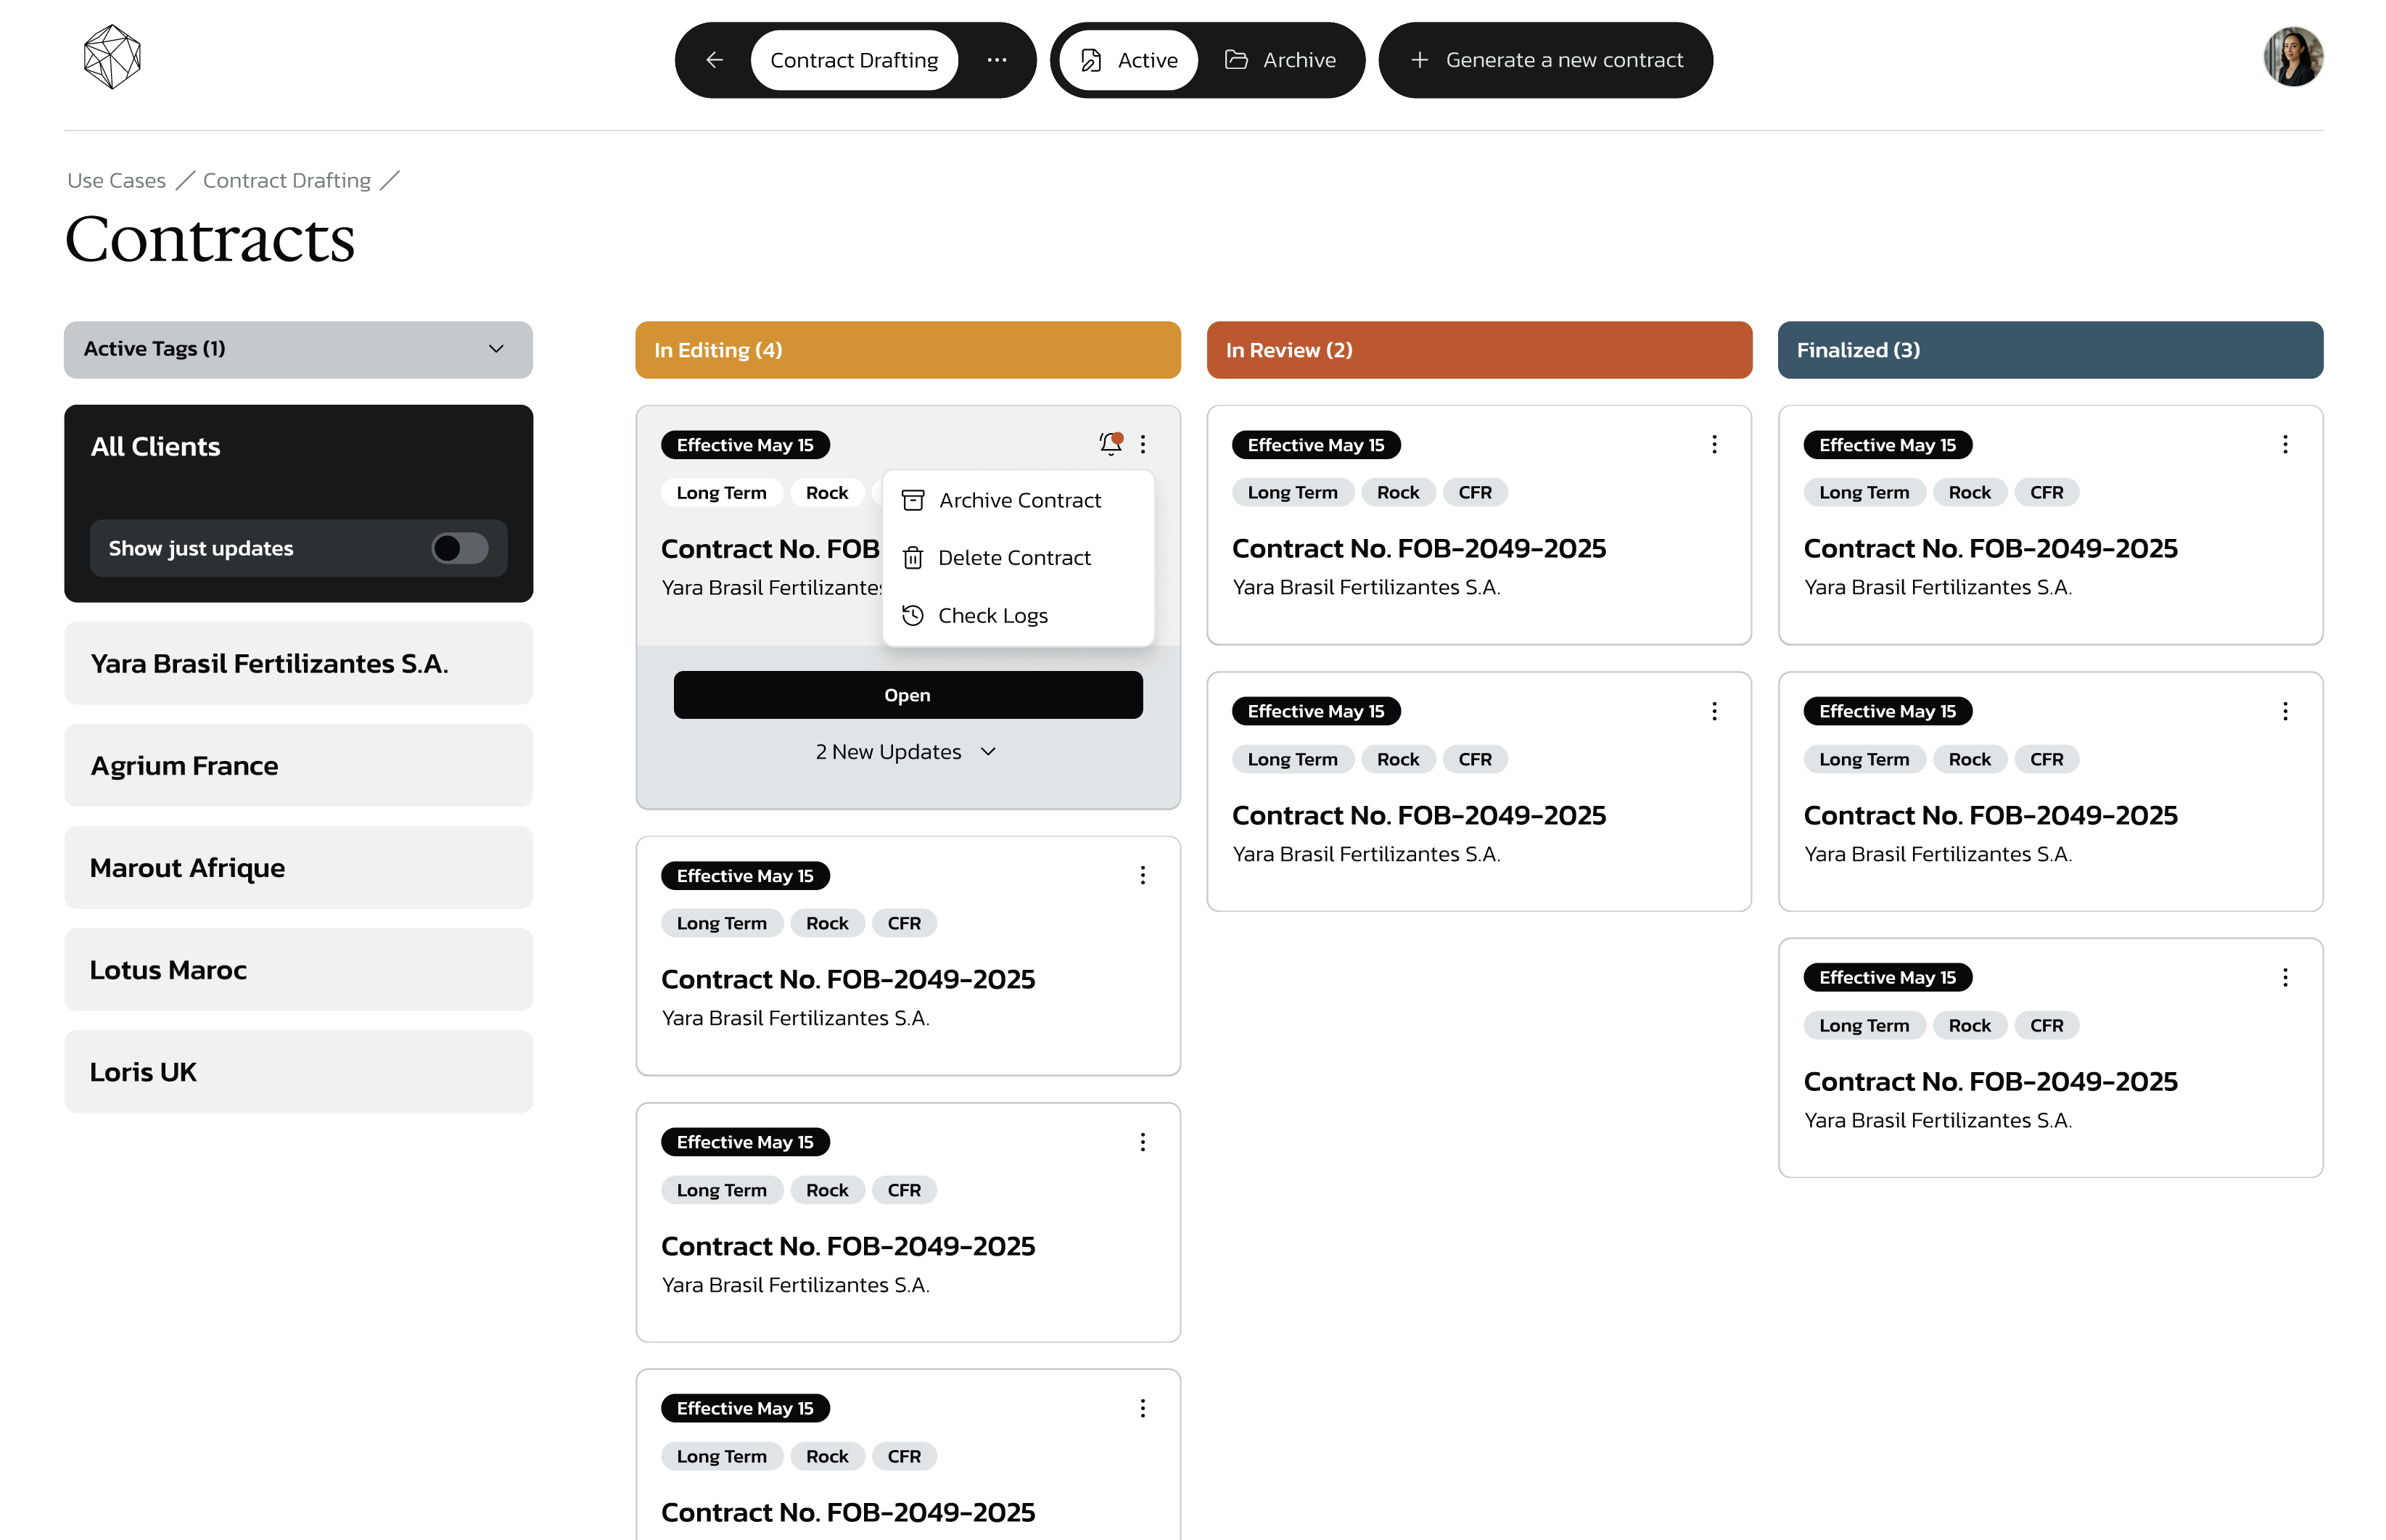
\includegraphics[width=1\textwidth]{Images/Contract Repository Page.png}
    \captionof{figure}{Contract Repository Interface}
    \label{fig:contract_repository_page}
\end{center}

% Contract Generation
\subsection{Contract Generation}
From the Contract Repository page, Sales users initiate contract creation via three input methods: audio recording, image uploads, or textual prompts. For instance, a user might prompt: \textit{\"Draft a spot contract for rock product with Incoterm CFR for new client Yara International\"}, optionally supplemented with additional image-based information.

\begin{center}
    \centering
    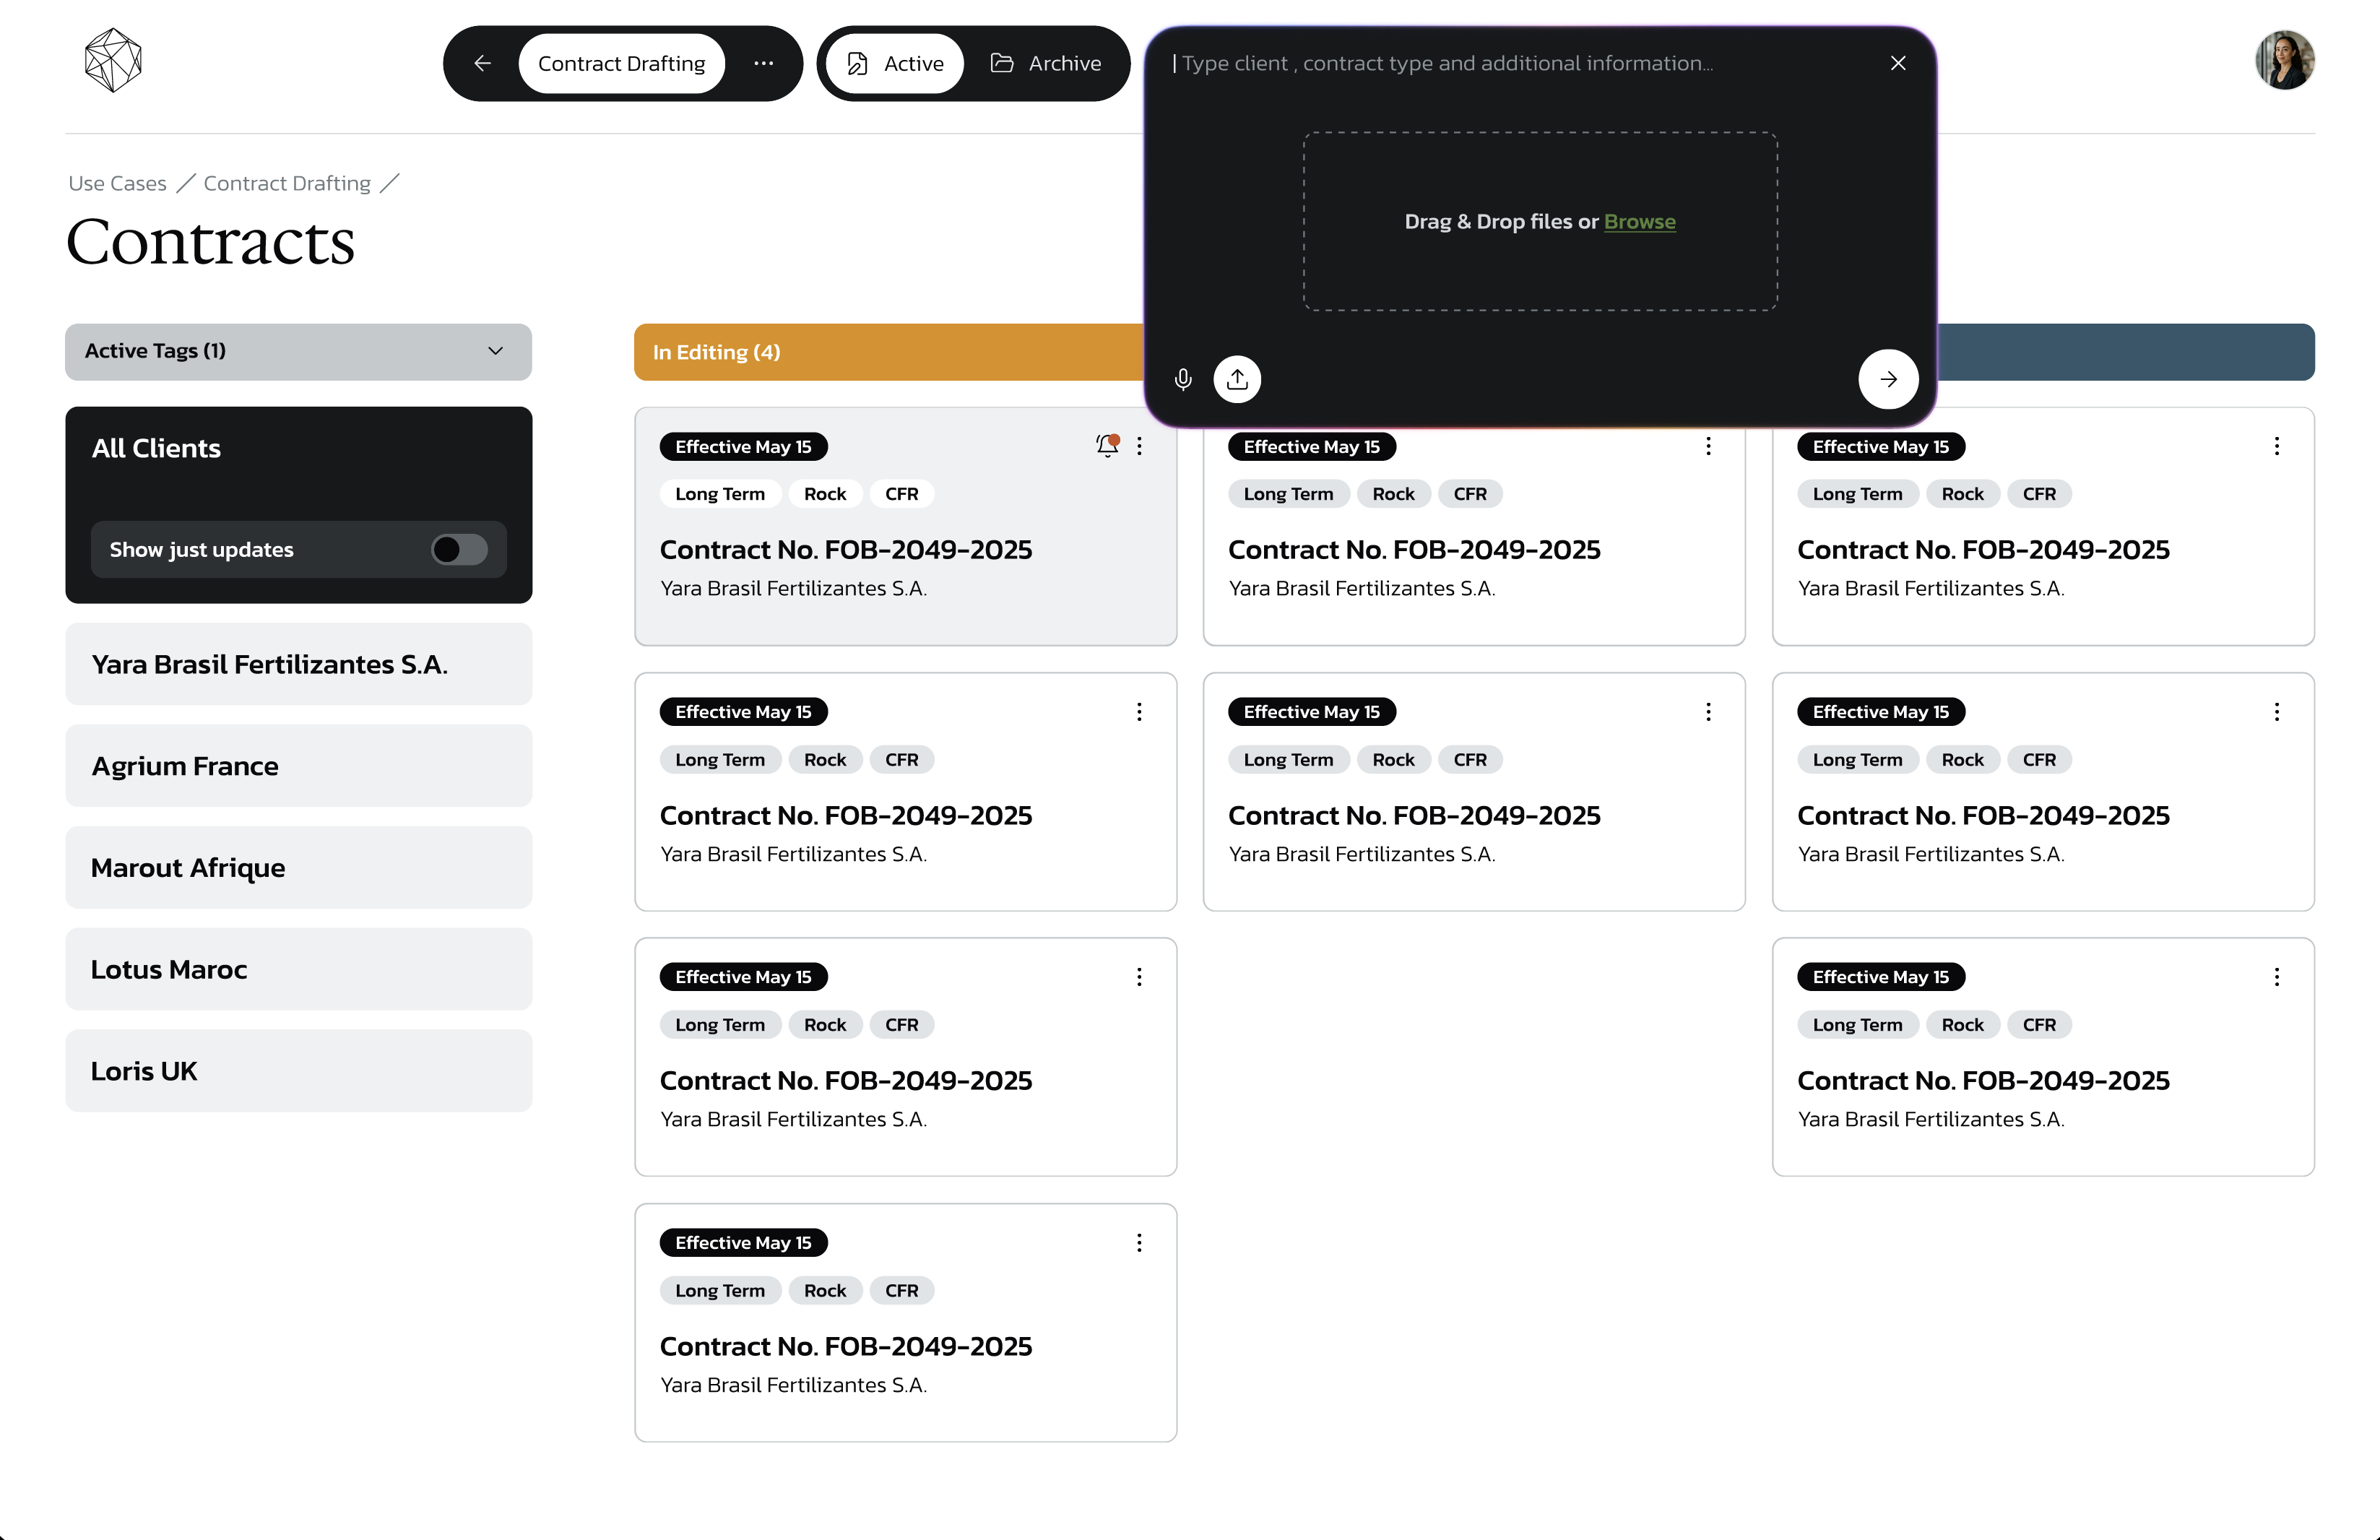
\includegraphics[width=1\textwidth]{Images/Generate Contract Component.png}
    \captionof{figure}{Contract Creation Component}
    \label{fig:contract_creation_component}
\end{center}

The first agent involved is the Generator, which initially checks for the required information: Contract Type, Incoterm, Client, and Product. Each combination of these fields corresponds to a distinct contract template. In the current scenario, the Generator detects that all essential fields are provided but identifies \textbf{Yara International} as a new client, not yet registered in the database. Consequently, the user is prompted either to confirm the new client details to avoid potential mismatches or, if the client already exists, to utilize an input field that suggests similar existing client names through Elasticsearch-based logic for selecting the correct one.

\begin{center}
    \centering
    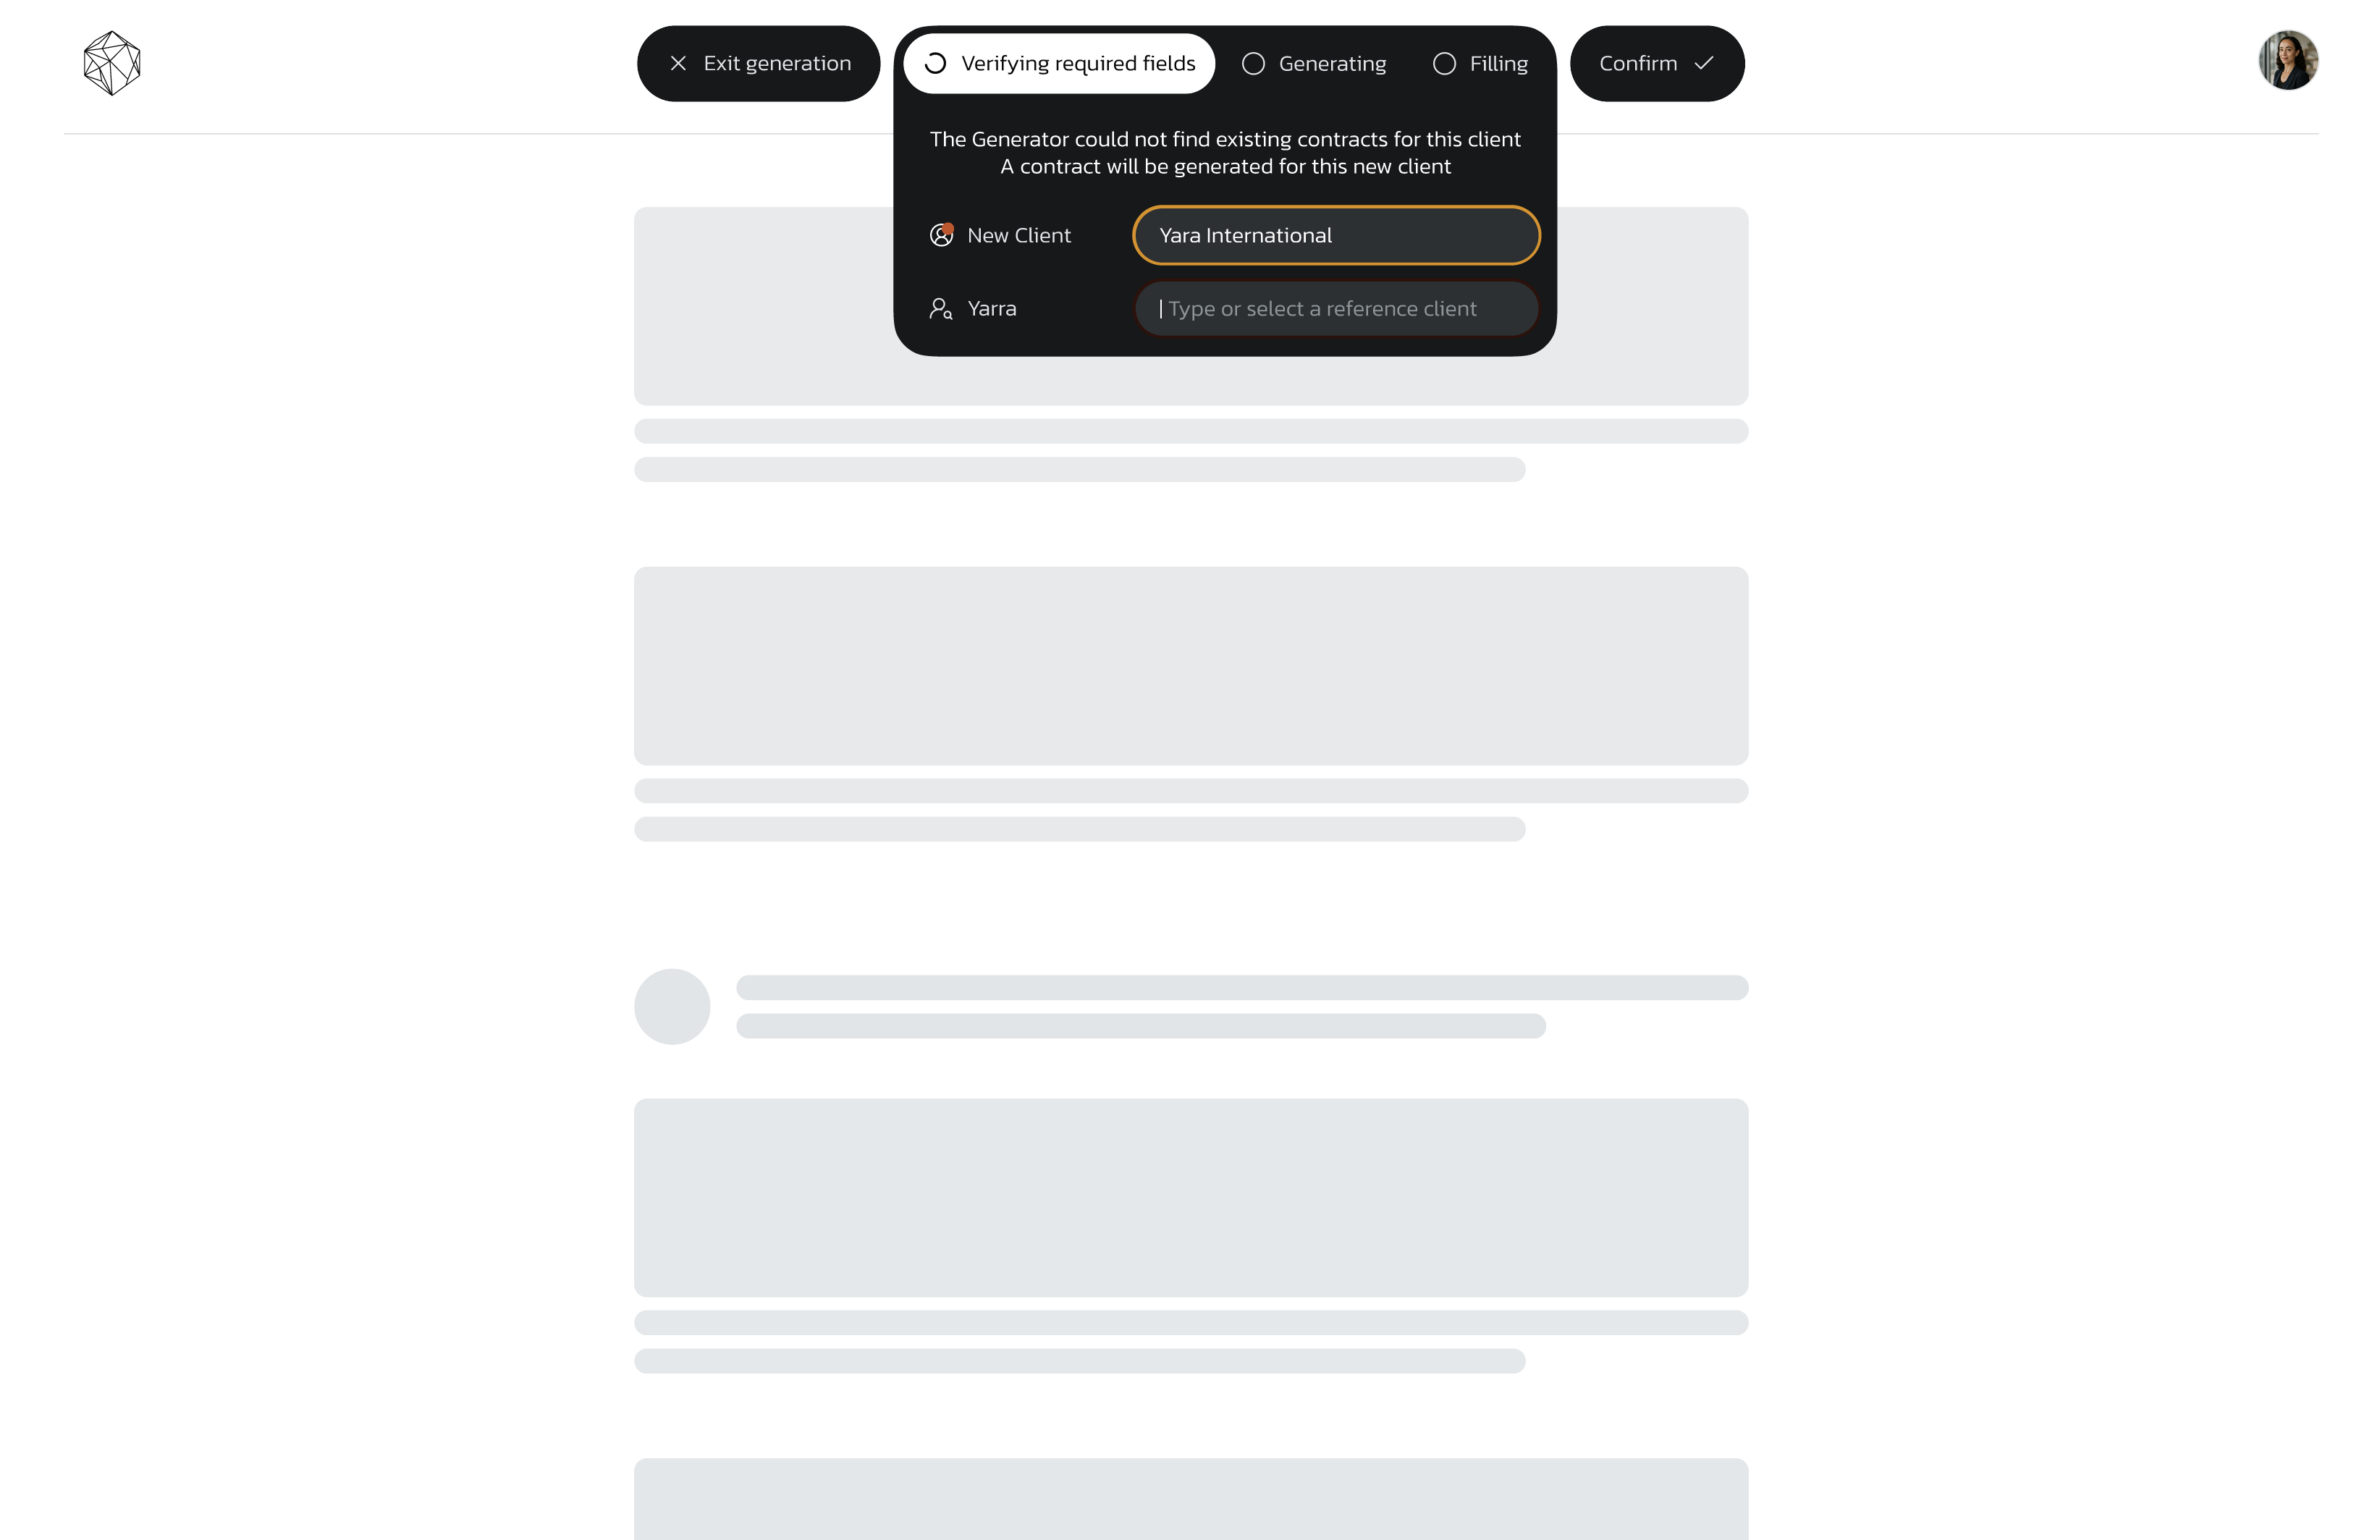
\includegraphics[width=1\textwidth]{Images/Generation Contract - Checking Required Fields.png}
    \captionof{figure}{Contract Verifying Fields Step}
    \label{fig:contract_verifying_fields_step}
\end{center}

The contract generation process involves the Generator agent, performing several key steps:

\begin{itemize}
    \item \textbf{Checking}: Confirms necessary fields (Contract Type, Incoterm, Client, Product) are provided. For new clients, users confirm client details or select from suggested matches using Elasticsearch.
    \item \textbf{Generating}: Creates contract sections and dynamically fills fields, leveraging historical data for existing clients to suggest relevant articles.
    \item \textbf{Filling}: Populates contract fields into respective database tables (Contracts, Contract Fields, Versions), and generates the initial contract version.
\end{itemize}

\begin{center}
    \centering
    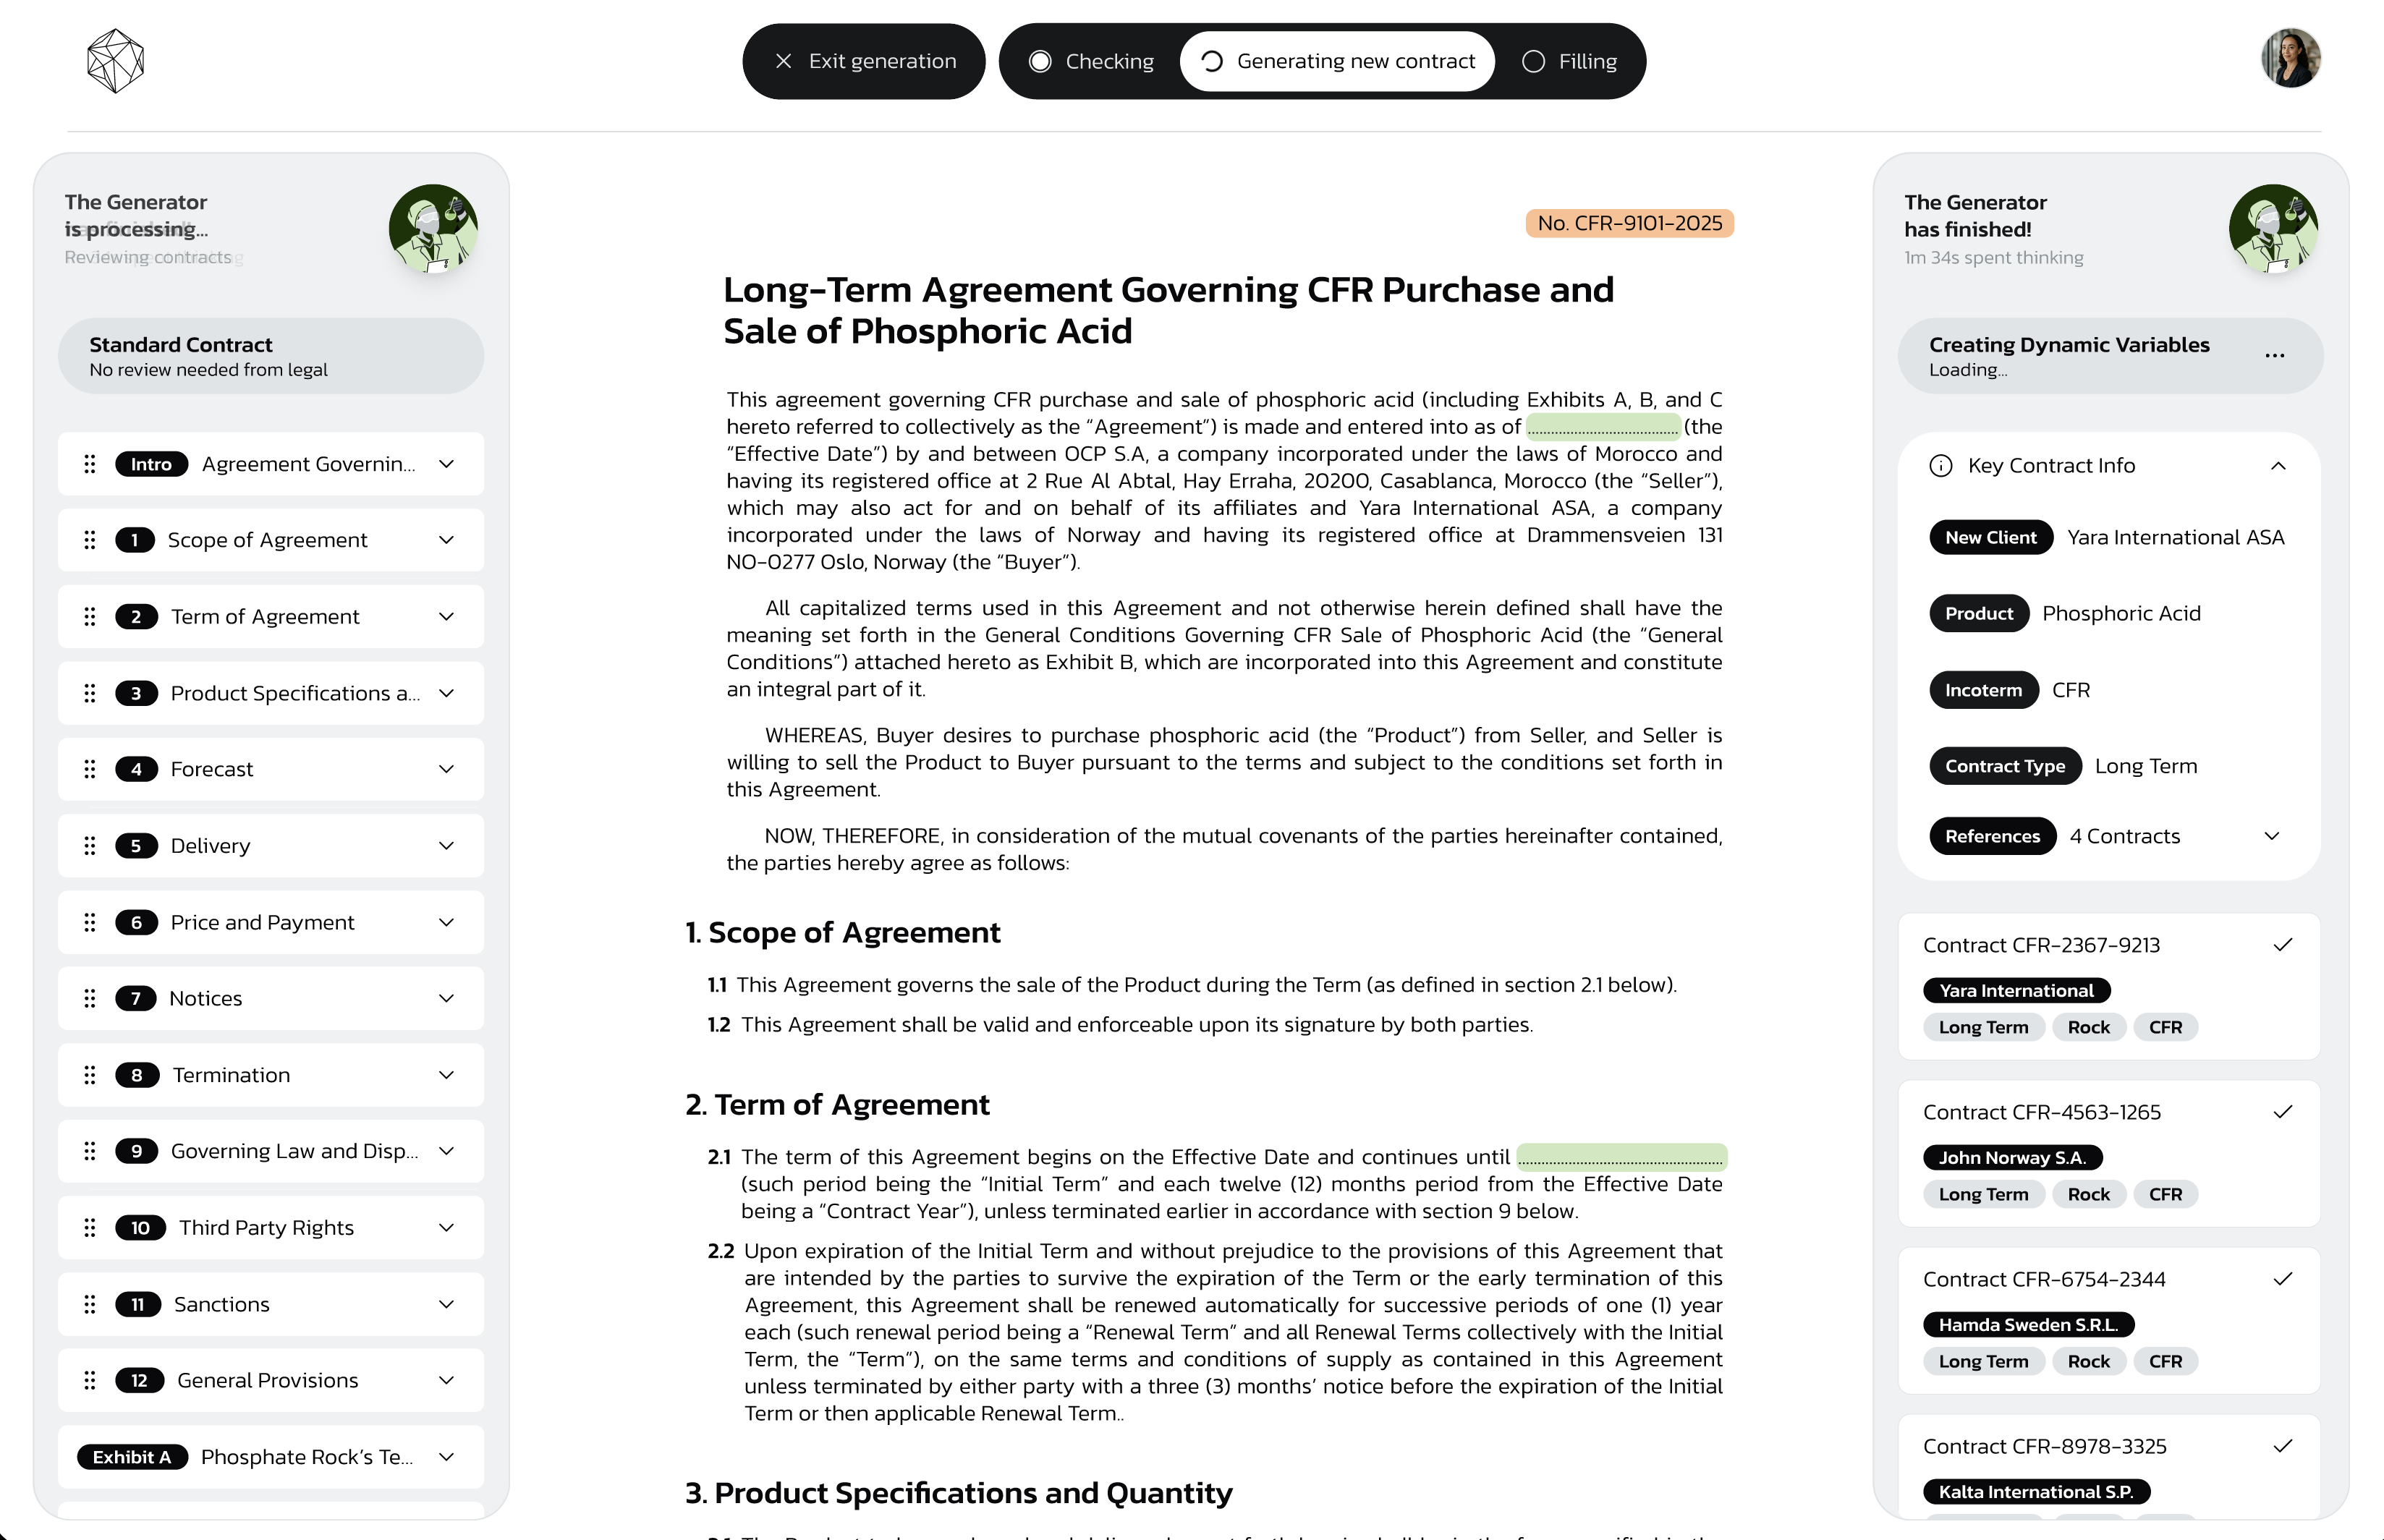
\includegraphics[width=1\textwidth]{Images/Generation Contract - Steps.png}
    \captionof{figure}{Contract Generating Process}
    \label{fig:contract_generation_steps}
\end{center}

% Contract Editor
\subsection{Contract Editor}
\begin{center}
    \centering
    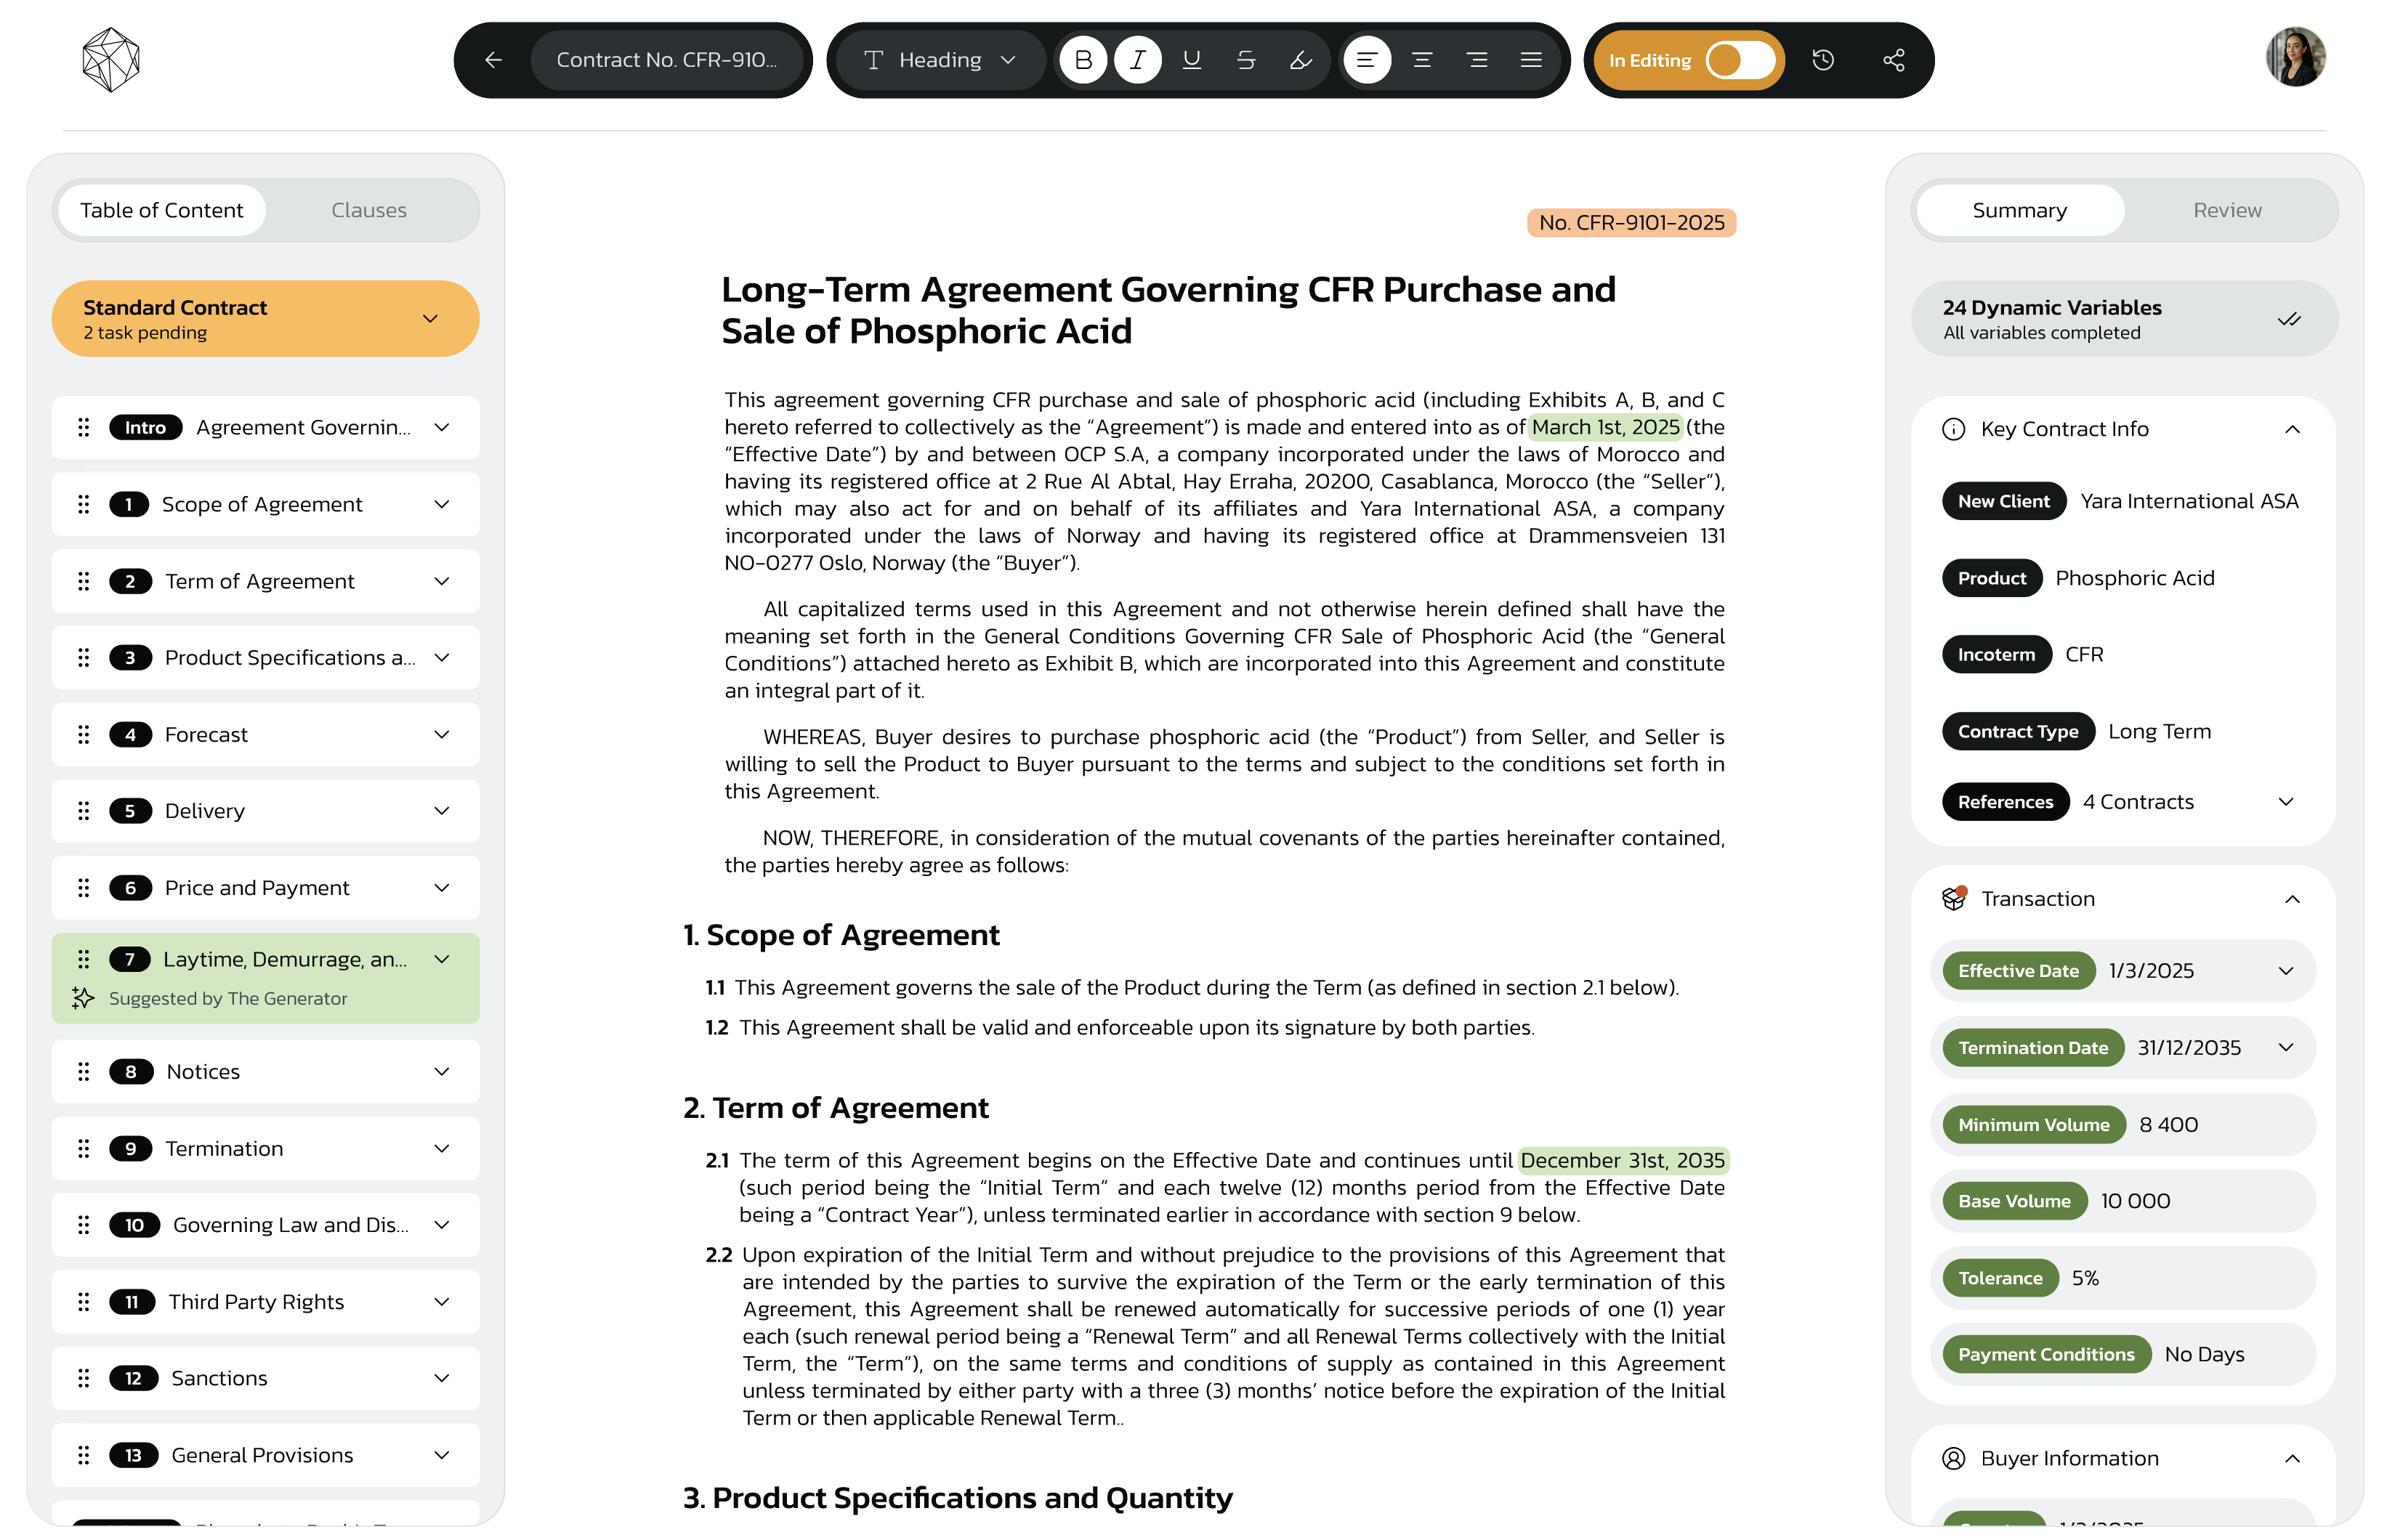
\includegraphics[width=1\textwidth]{Images/Contract Editor Page.png}
    \captionof{figure}{Contract Editor Interface}
    \label{fig:contract_editor_page}
\end{center}

Upon creation or selection from the repository, the contract opens in the Contract Editor interface, structured into four distinct sections:

\begin{itemize}
    \item \textbf{Header:} The header section prominently displays the platform logo on the left and the user profile logo on the right, which provides quick access for modifying user information or logging out. Centrally located within the header, the contract title is editable directly by the user. Navigation controls are positioned alongside the title, including a button to return to the Contract Repository page. Additionally, a formatting toolbar allows users to apply text styles such as bold, italic, or underline. To the right side of the toolbar, three action buttons facilitate contract status updates, history access, and contract sharing options.
    \item \textbf{Left Panel:} This panel provides easy navigation through the document's structured contents with a dynamic table of contents. Additionally, it contains functionalities for managing contract clauses, including viewing existing clauses, requesting new ones, or initiating clause modifications.
    \item \textbf{Right Panel:} The right panel consists of two critical components. First, the summary panel, which lists all required and dynamic fields of the contract, allowing users to edit these directly. Second, the review panel where the Reviewer Agent performs comprehensive reviews, ensuring accuracy, consistency, and compliance with regulatory standards.
    \item \textbf{Editor Body:} At the heart of the interface lies the document editing area, powered by the Tiptap editor. This editor allows Legal users full editing capabilities to draft, modify, and finalize the contract's textual content. For Sales users, the editor body is presented in a read-only mode, ensuring document integrity and maintaining clear responsibilities between roles.
\end{itemize}

% AI-Suggested Articles
\subsubsection{AI-Suggested Articles}
The Generator agent may suggest relevant articles based on past client contracts or user-specified historical references. Users can accept or reject suggestions, automatically integrating accepted articles into the editor.

\begin{center}
    \centering
    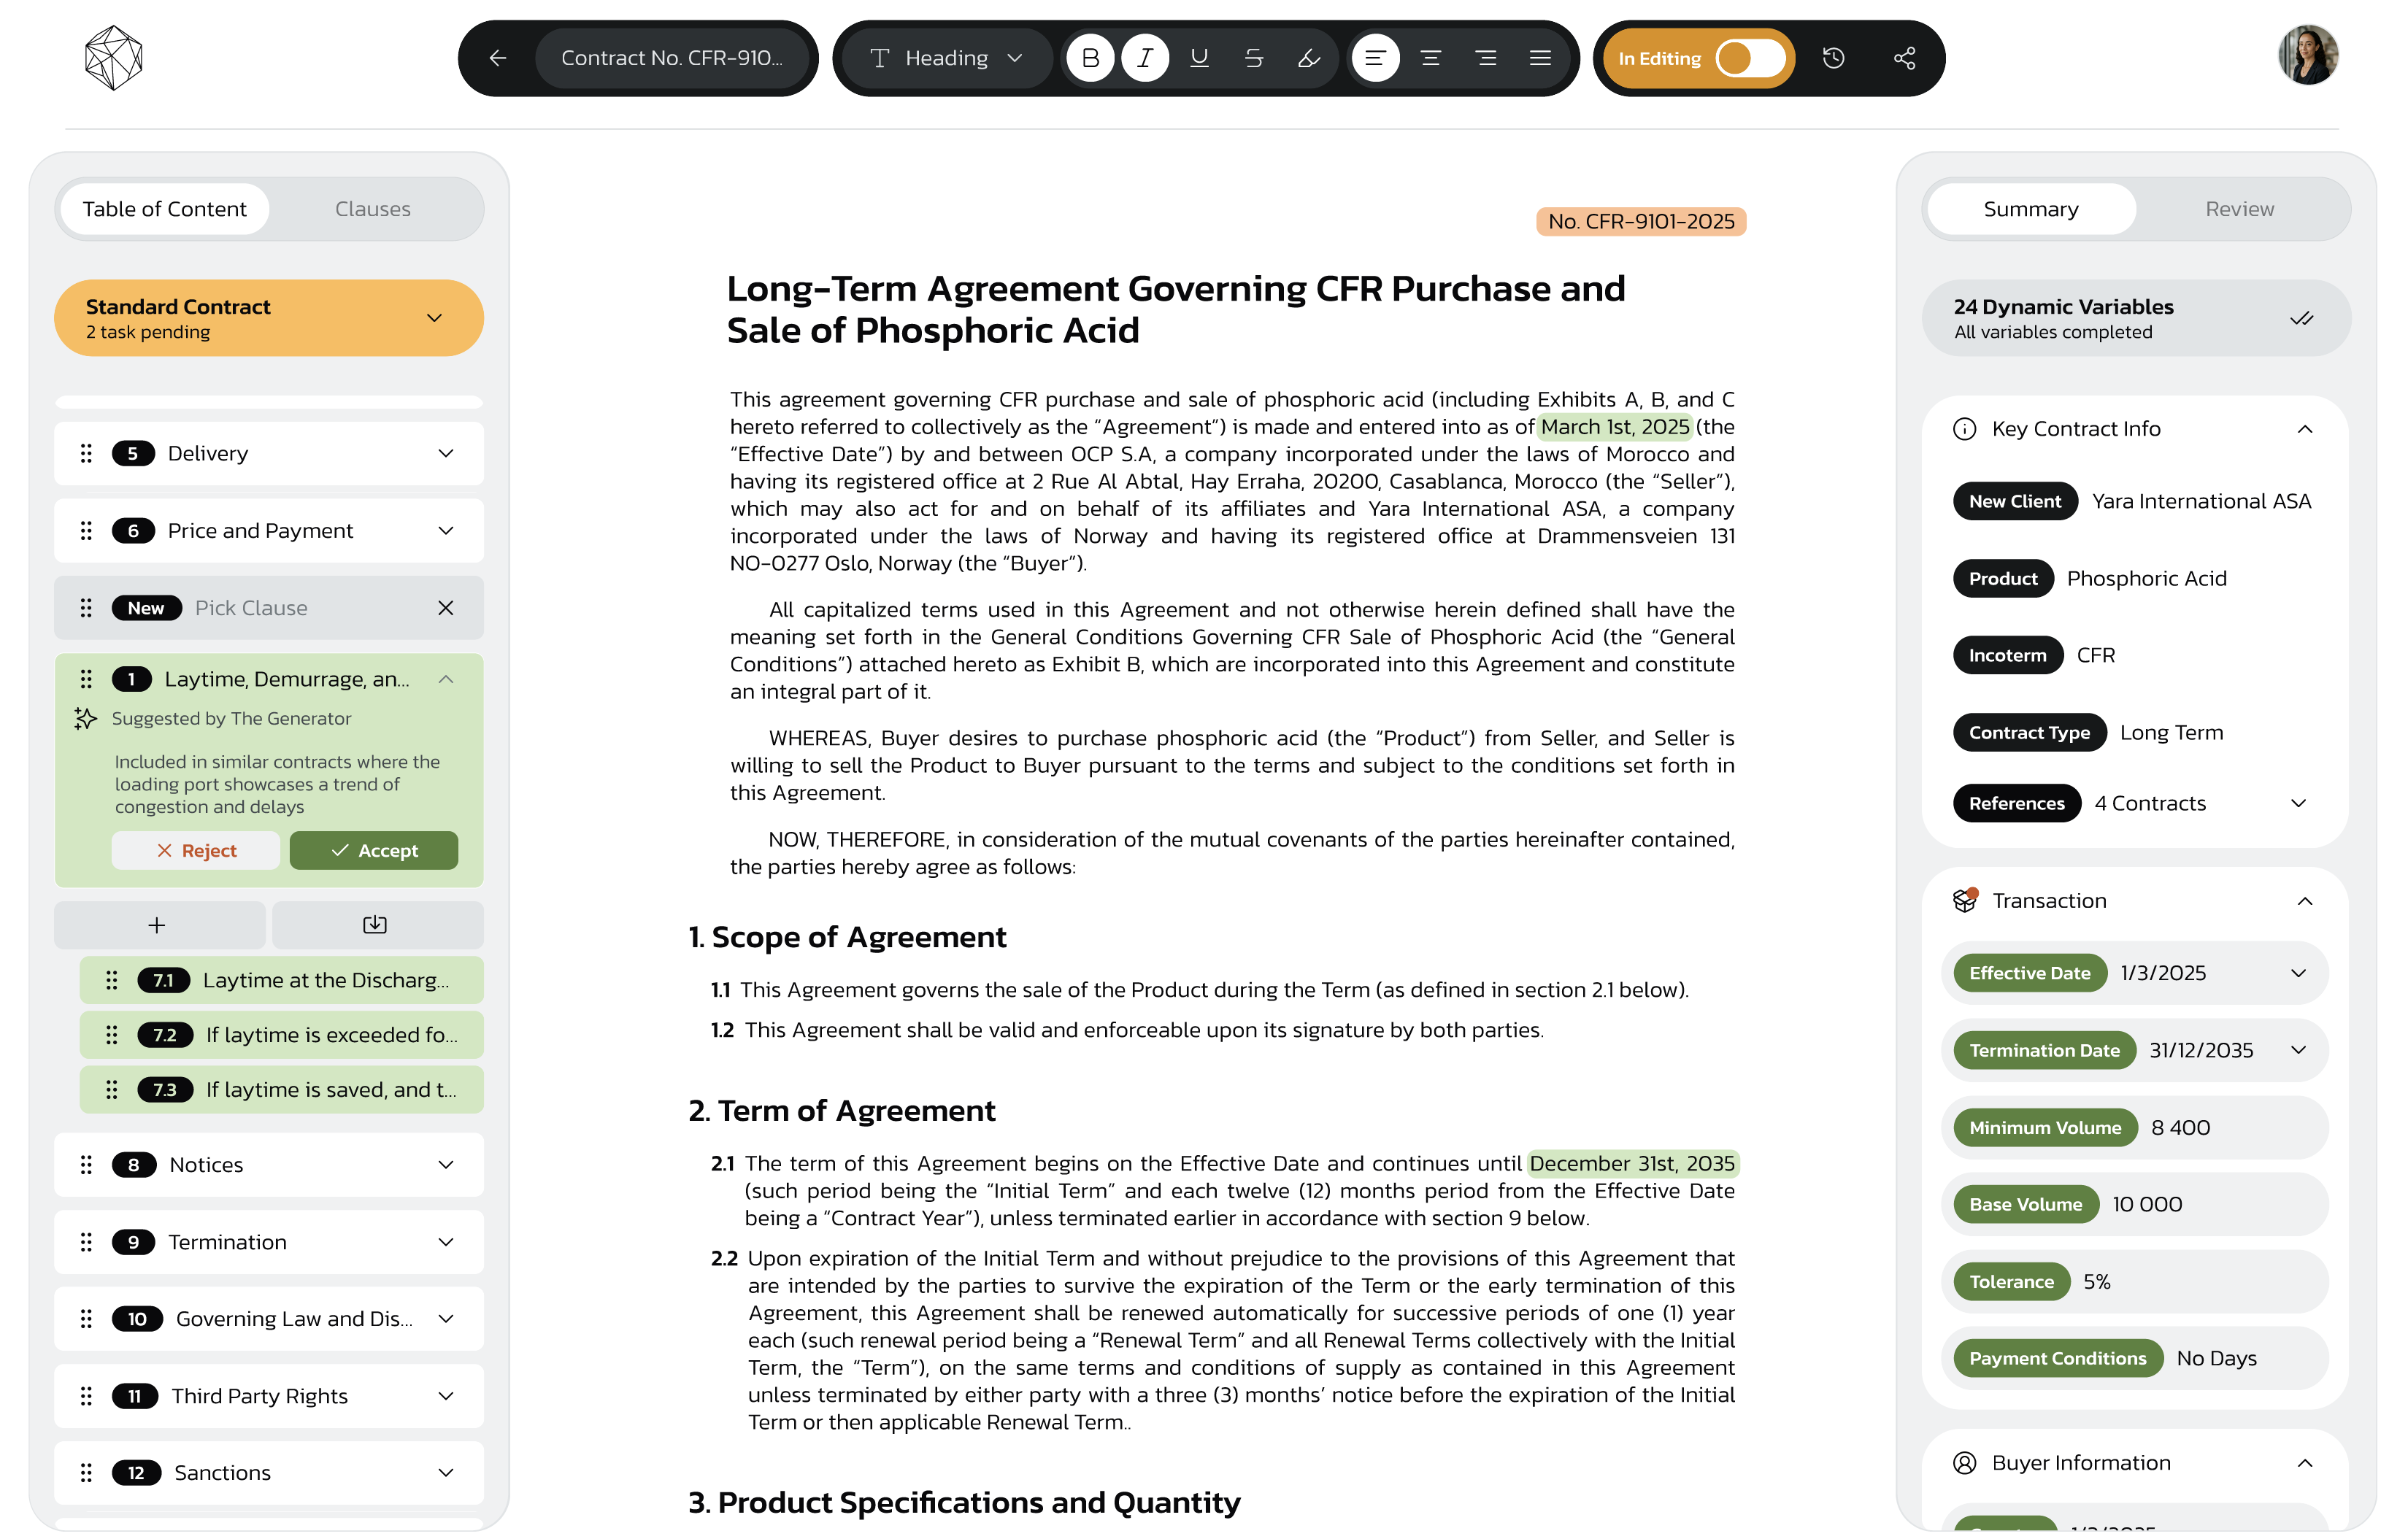
\includegraphics[width=1\textwidth]{Images/Article Suggested By Agent.png}
    \captionof{figure}{Contract Editor with AI-Suggested Article}
    \label{fig:article_suggested_by_agent}
\end{center}

% Clause Management
\subsubsection{Clause Management}

As Sales users are restricted from directly editing contracts, the platform provides a specialized clause management feature to facilitate necessary modifications through clause requests. When a Sales user identifies a need to modify a contract, they initiate a new clause request. This action can be triggered through multiple methods: directly via the "New Clause" button in the left panel, by selecting a specific section within the contract to associate the request with the content and its number, or through interaction with existing comments within the editor interface.

\begin{center}
    \centering
    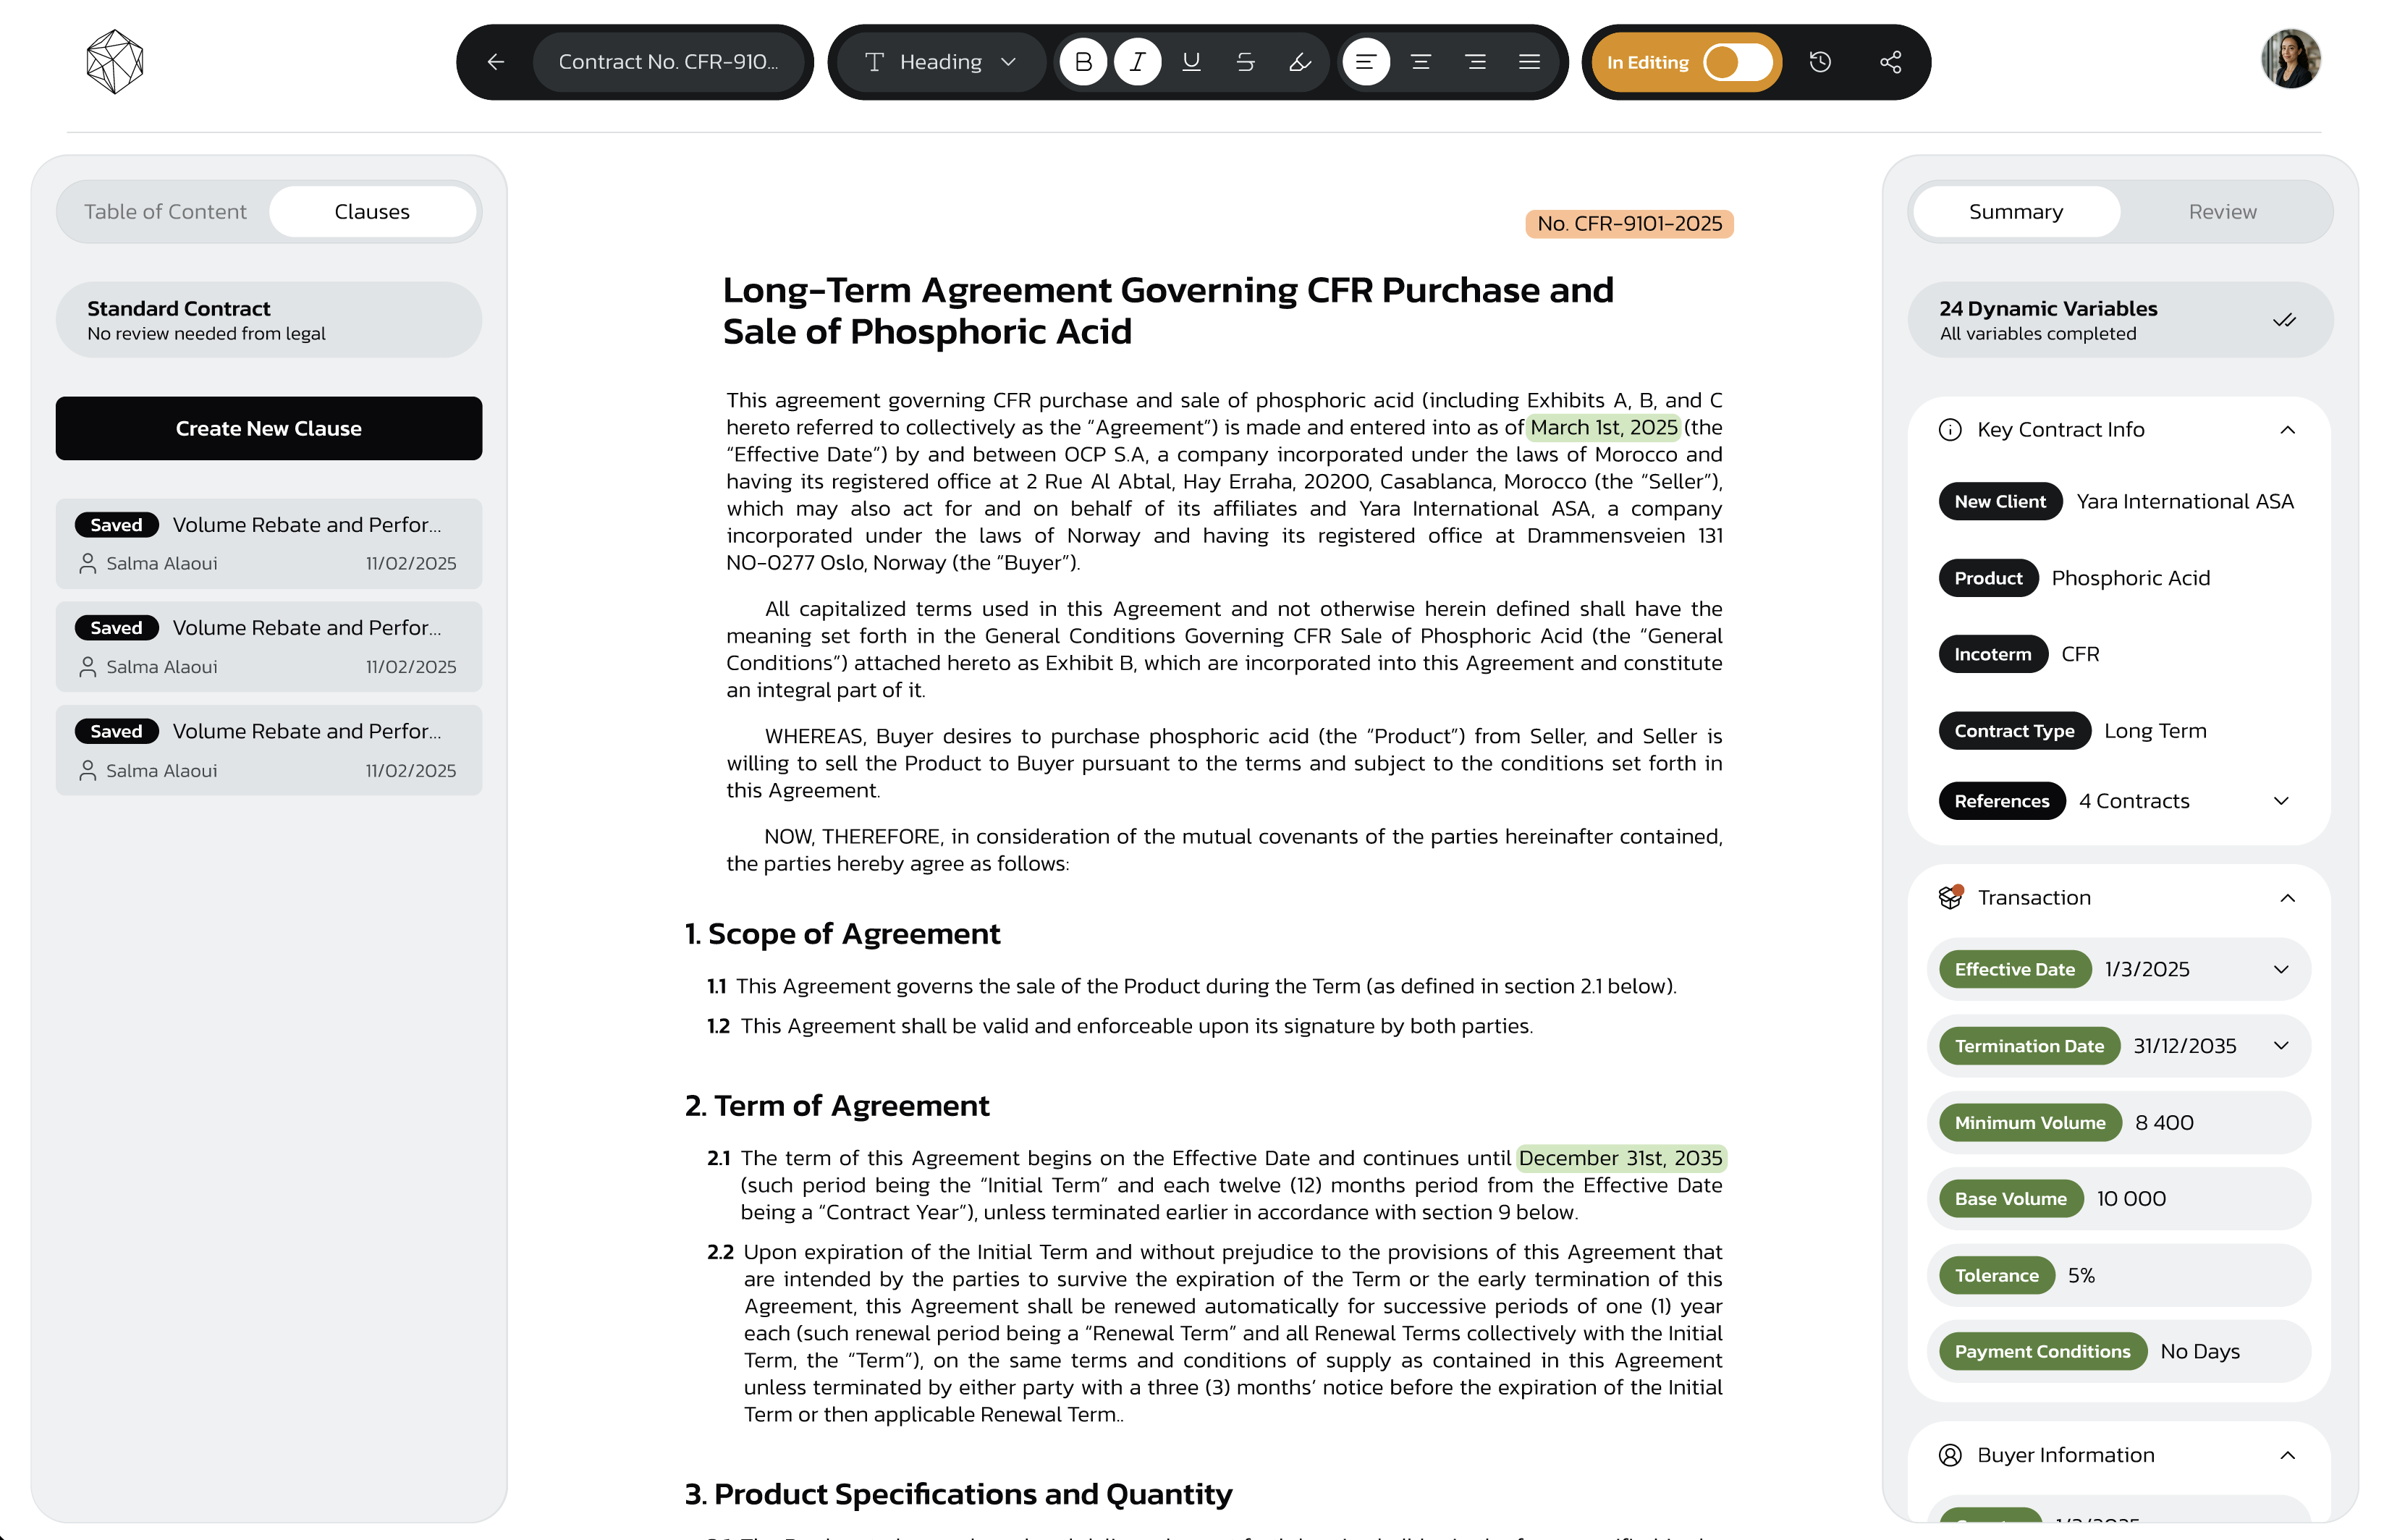
\includegraphics[width=1\textwidth]{Images/Clause Requests - Create New Clause.png}
    \captionof{figure}{Clause Request Interface}
    \label{fig:create_clause_request}
\end{center}

\begin{center}
    \centering
    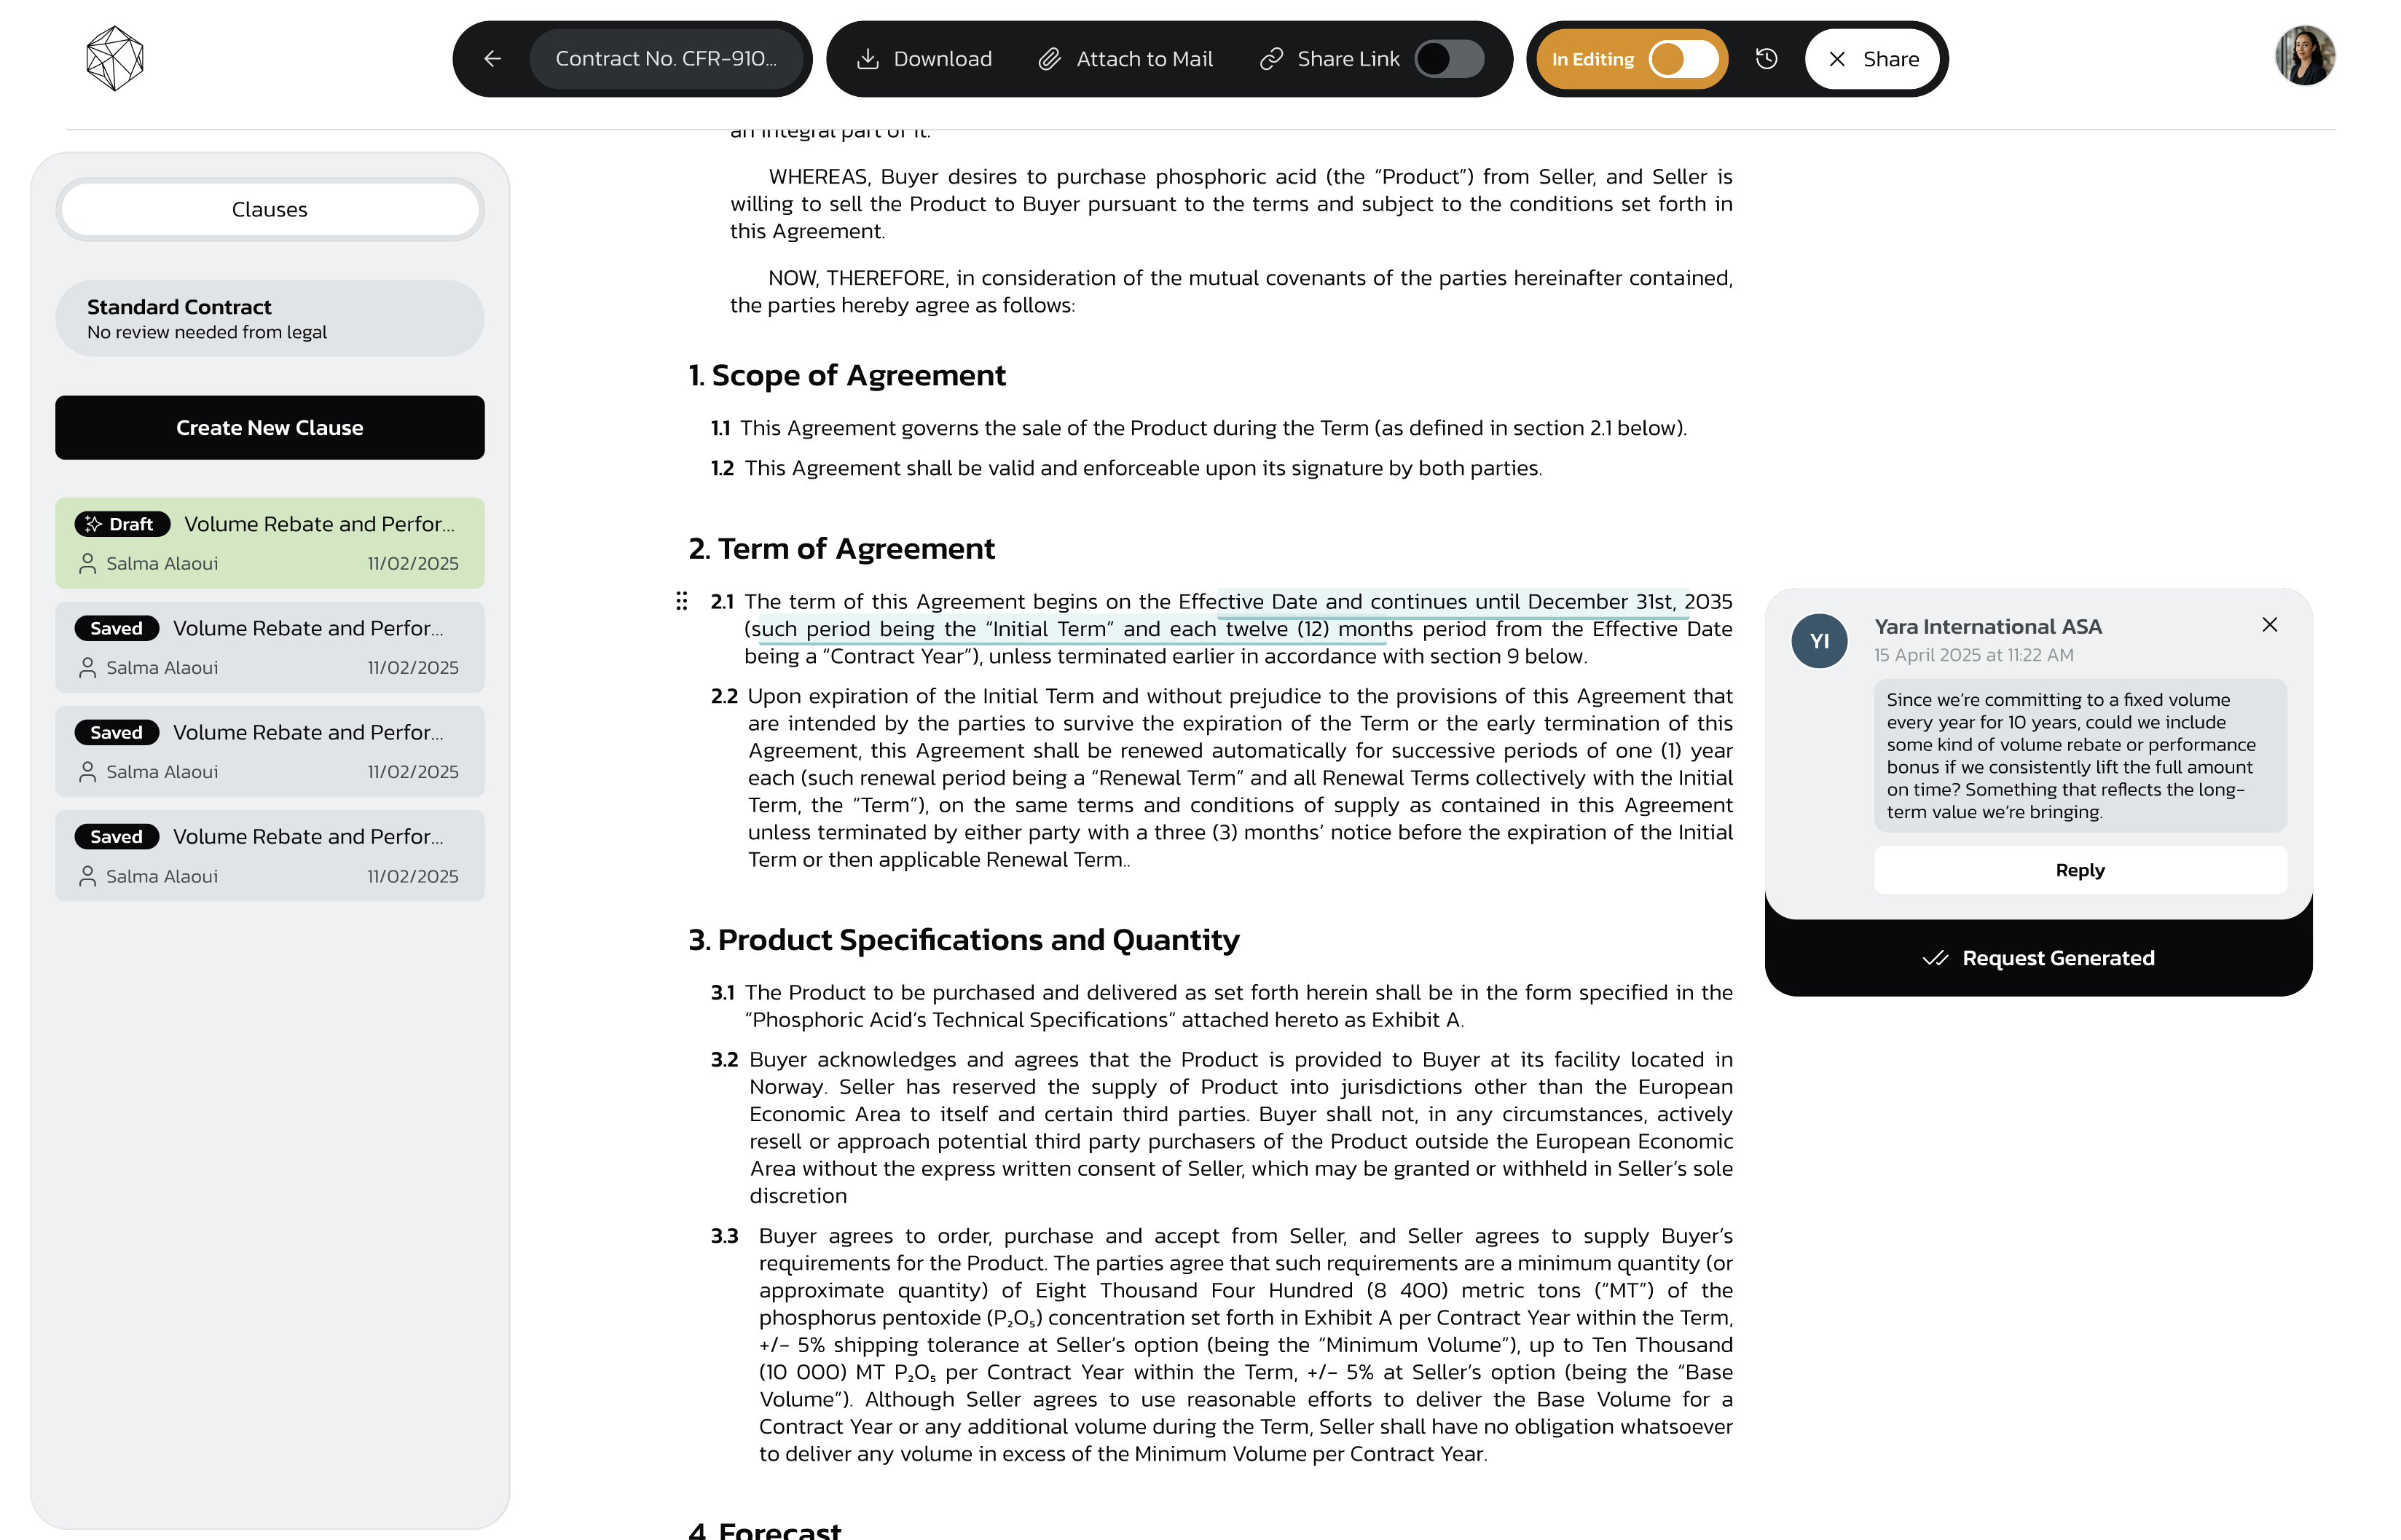
\includegraphics[width=1\textwidth]{Images/Clause Requests - Create New Clause from a comment.png}
    \captionof{figure}{Create New Clause from Comment}
    \label{fig:create_clause_request_from_comment}
\end{center}

Upon initiating a clause request, Sales users compose a detailed description of their desired modification. To enhance clarity and precision, the platform provides multiple input options, including voice recordings, file uploads, and insertion of dynamic fields using the "@" symbol. Additionally, users can refine their descriptions utilizing integrated LLM assistance, ensuring the request accurately communicates the intended modifications.

\begin{center}
    \centering
    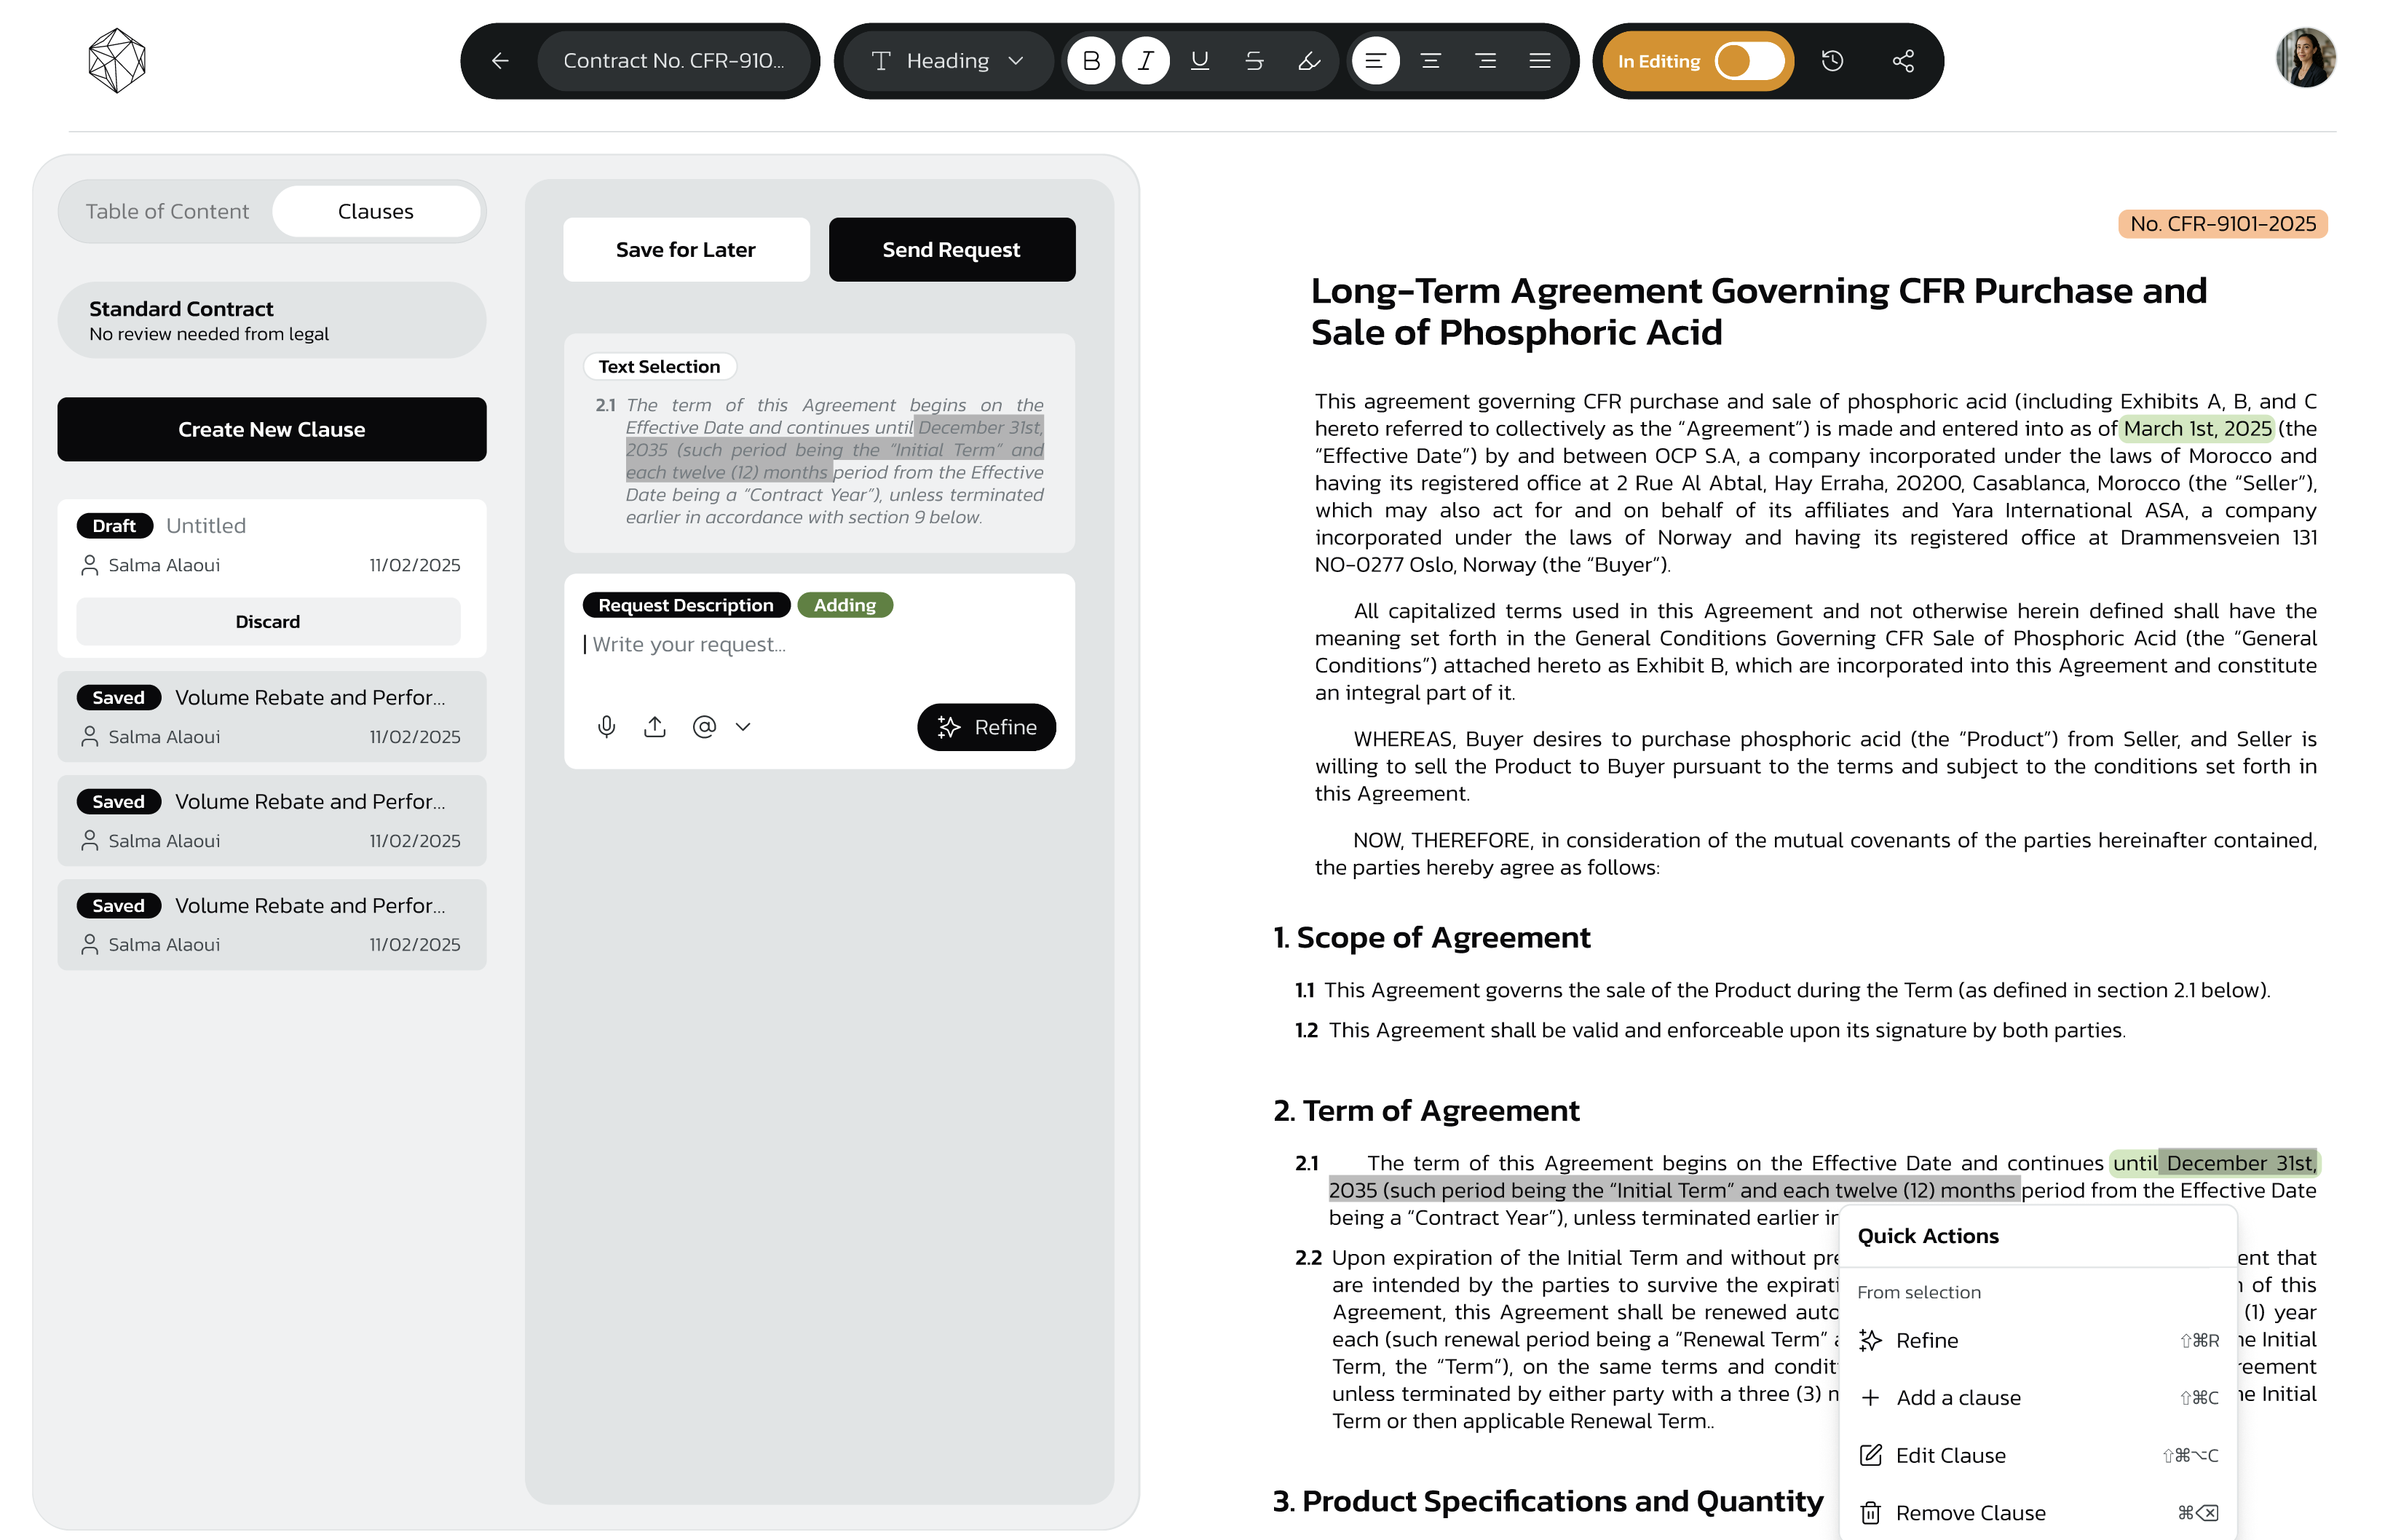
\includegraphics[width=1\textwidth]{Images/Clause Requests - Clause Description.png}
    \captionof{figure}{Clause Request Description and Enhancement}
    \label{fig:clause_request_description}
\end{center}

After submission, the Legal team receives a notification indicating the clause request along with details of the Sales user who submitted it. Upon reviewing the notification, Legal users access the clause management interface to review the Sales user's request comprehensively. This interface provides a dedicated editor enabling Legal users to add, modify, or delete clauses and subclauses directly. The editor also includes the same capabilities provided to Sales users, such as refining with LLM assistance, voice recording, and file uploads. Legal users can finalize their changes immediately or save their edits for later completion.

\begin{center}
    \centering
    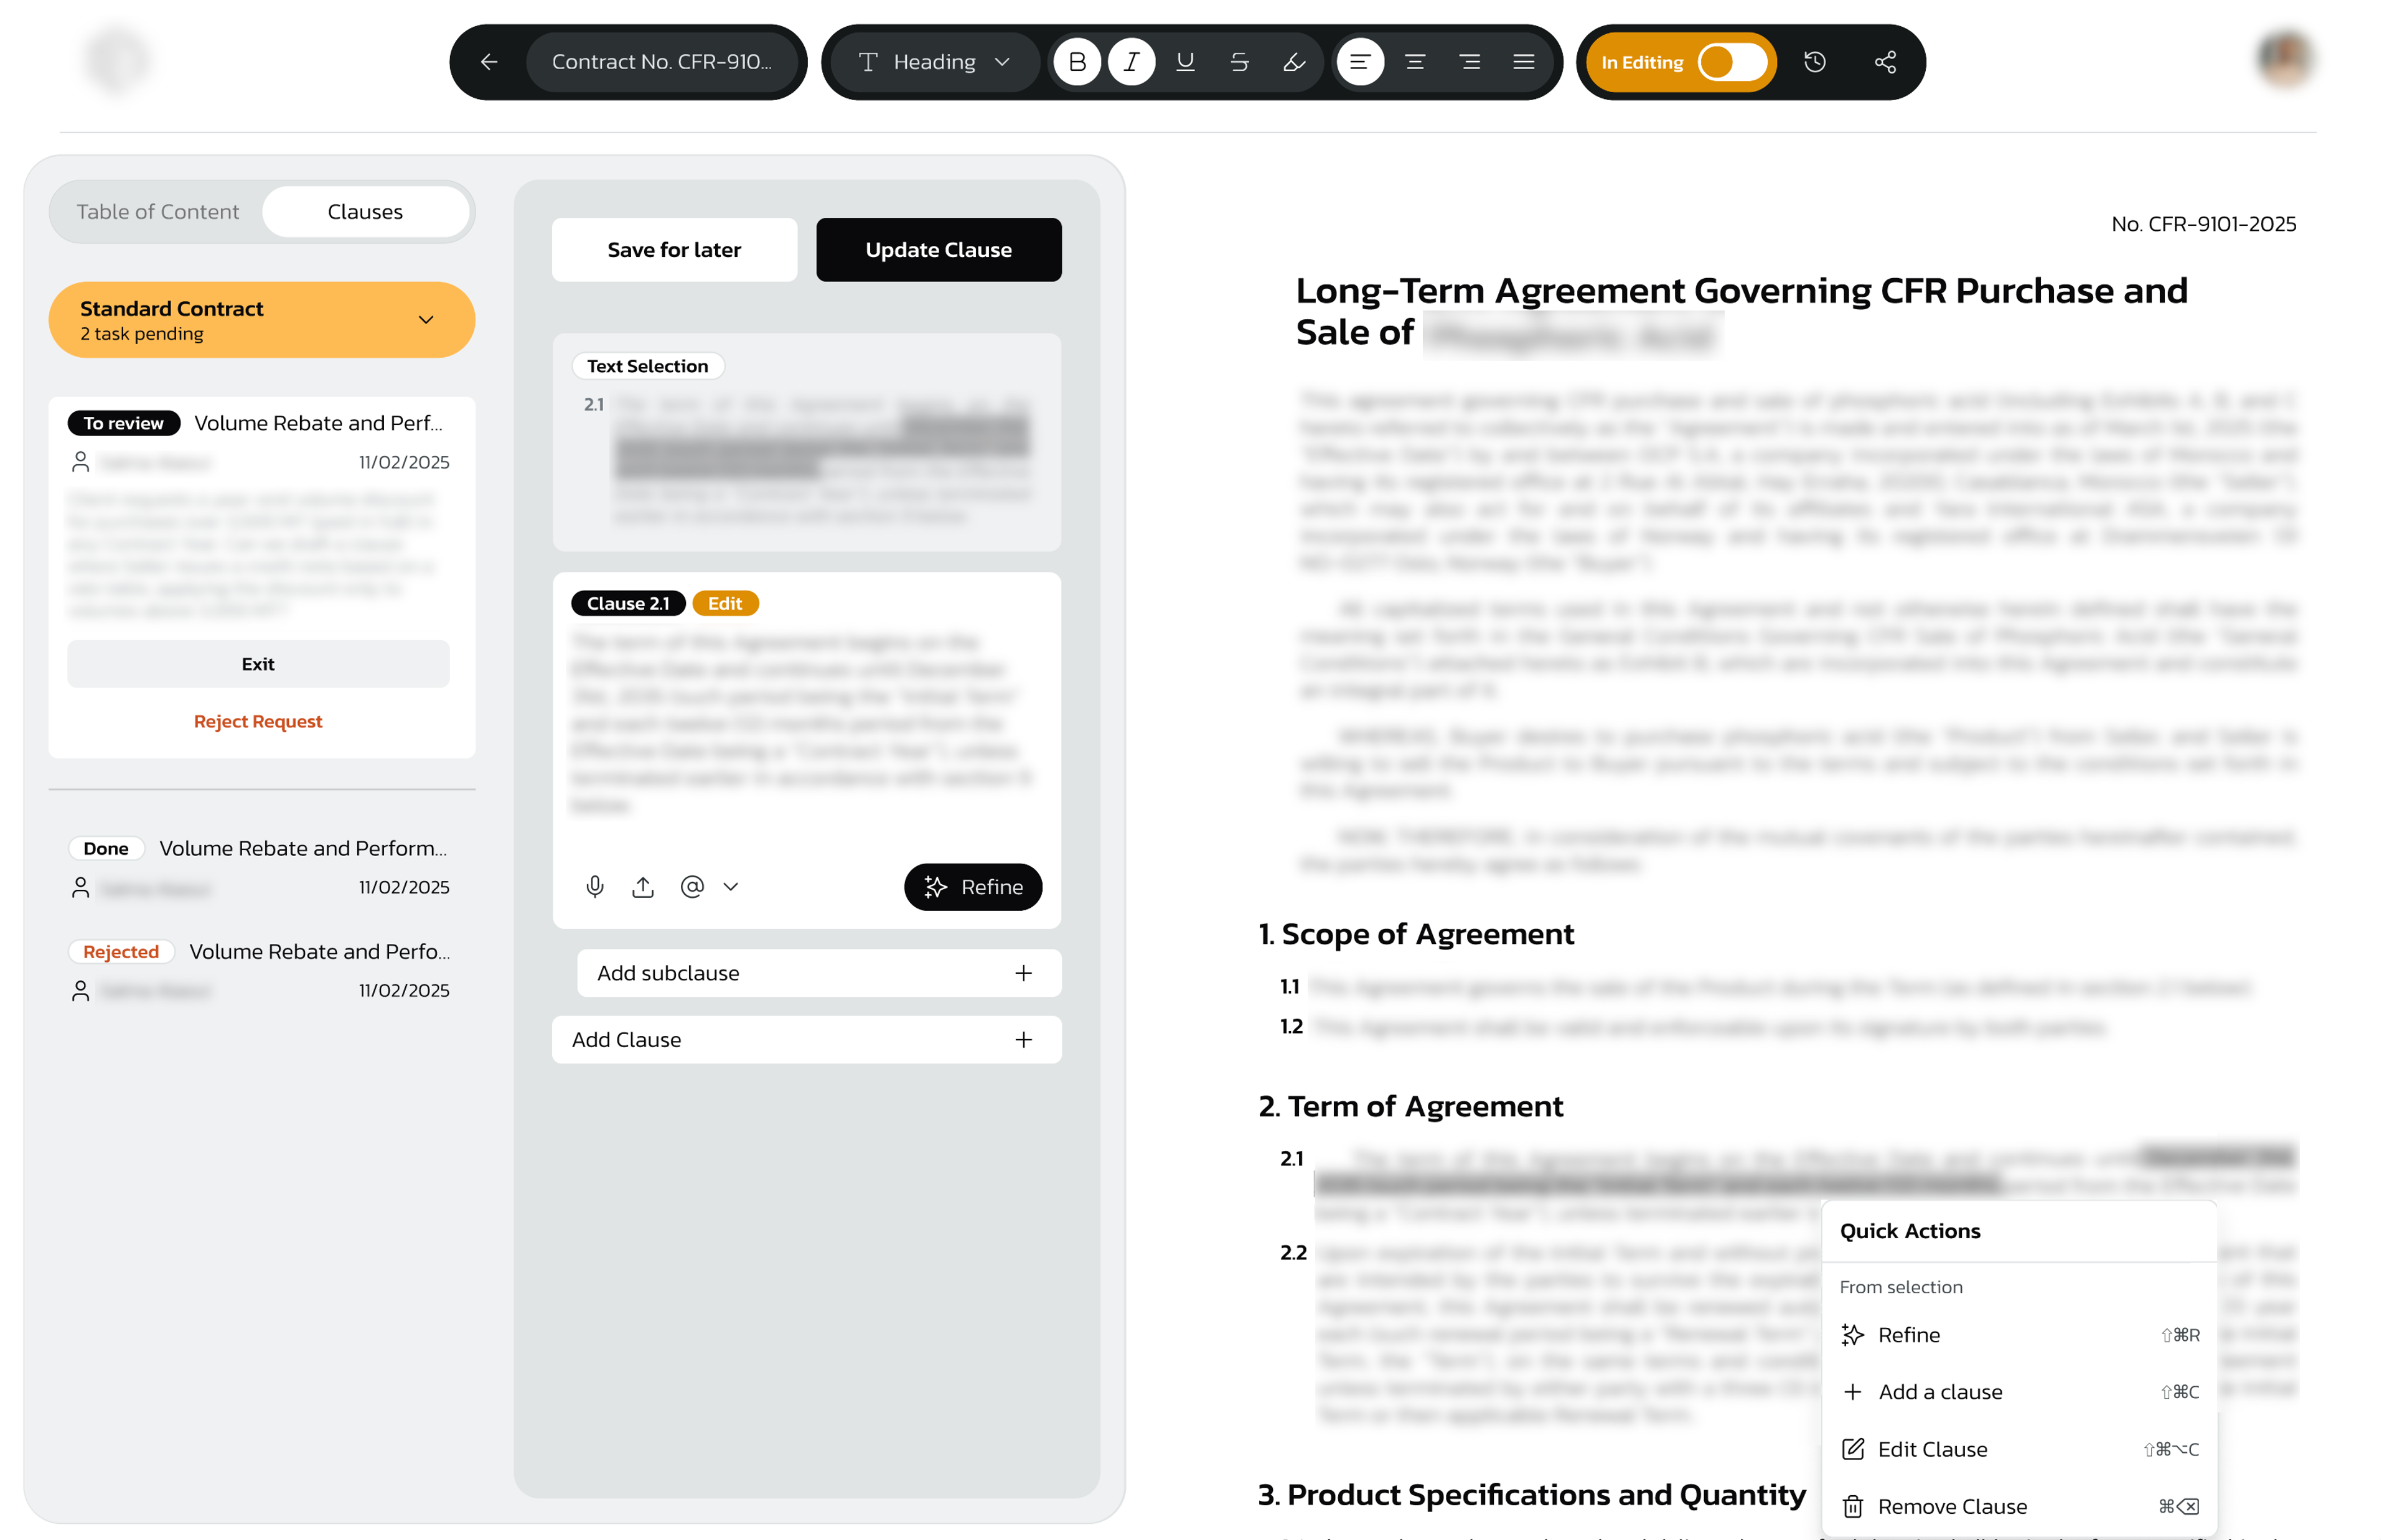
\includegraphics[width=1\textwidth]{Images/Clause Requests - Respond to a Request.png}
    \captionof{figure}{Clause Request Review Interface}
    \label{fig:clause_request_review_interface}
\end{center}

% Contract Review
\subsection{Contract Review}
Upon marking a contract as \textit{"In Review"} by Sales users, Legal users can initiate a thorough review either manually or through AI-driven assistance. Two specialized AI agents are available for this purpose:

\begin{itemize}
    \item \textbf{Reviewer Agent:} Conducts Data Accuracy and Consistency checks, verifying essential details such as dates, amounts, and product specifications. It also evaluates text clarity, grammar, and formatting consistency.
    \item \textbf{Guardian Agent:} Performs comprehensive Legal Security evaluations, ensuring compliance with legal standards, verifying clauses, payment terms, Incoterms responsibilities, and detecting deviations from predefined templates.
\end{itemize}

Upon execution, the Reviewer agent provides an overall quality score with targeted suggestions to enhance the contract. Legal users can iteratively apply these recommendations, aiming to achieve optimal compliance (100\%).

\begin{center}
    \centering
    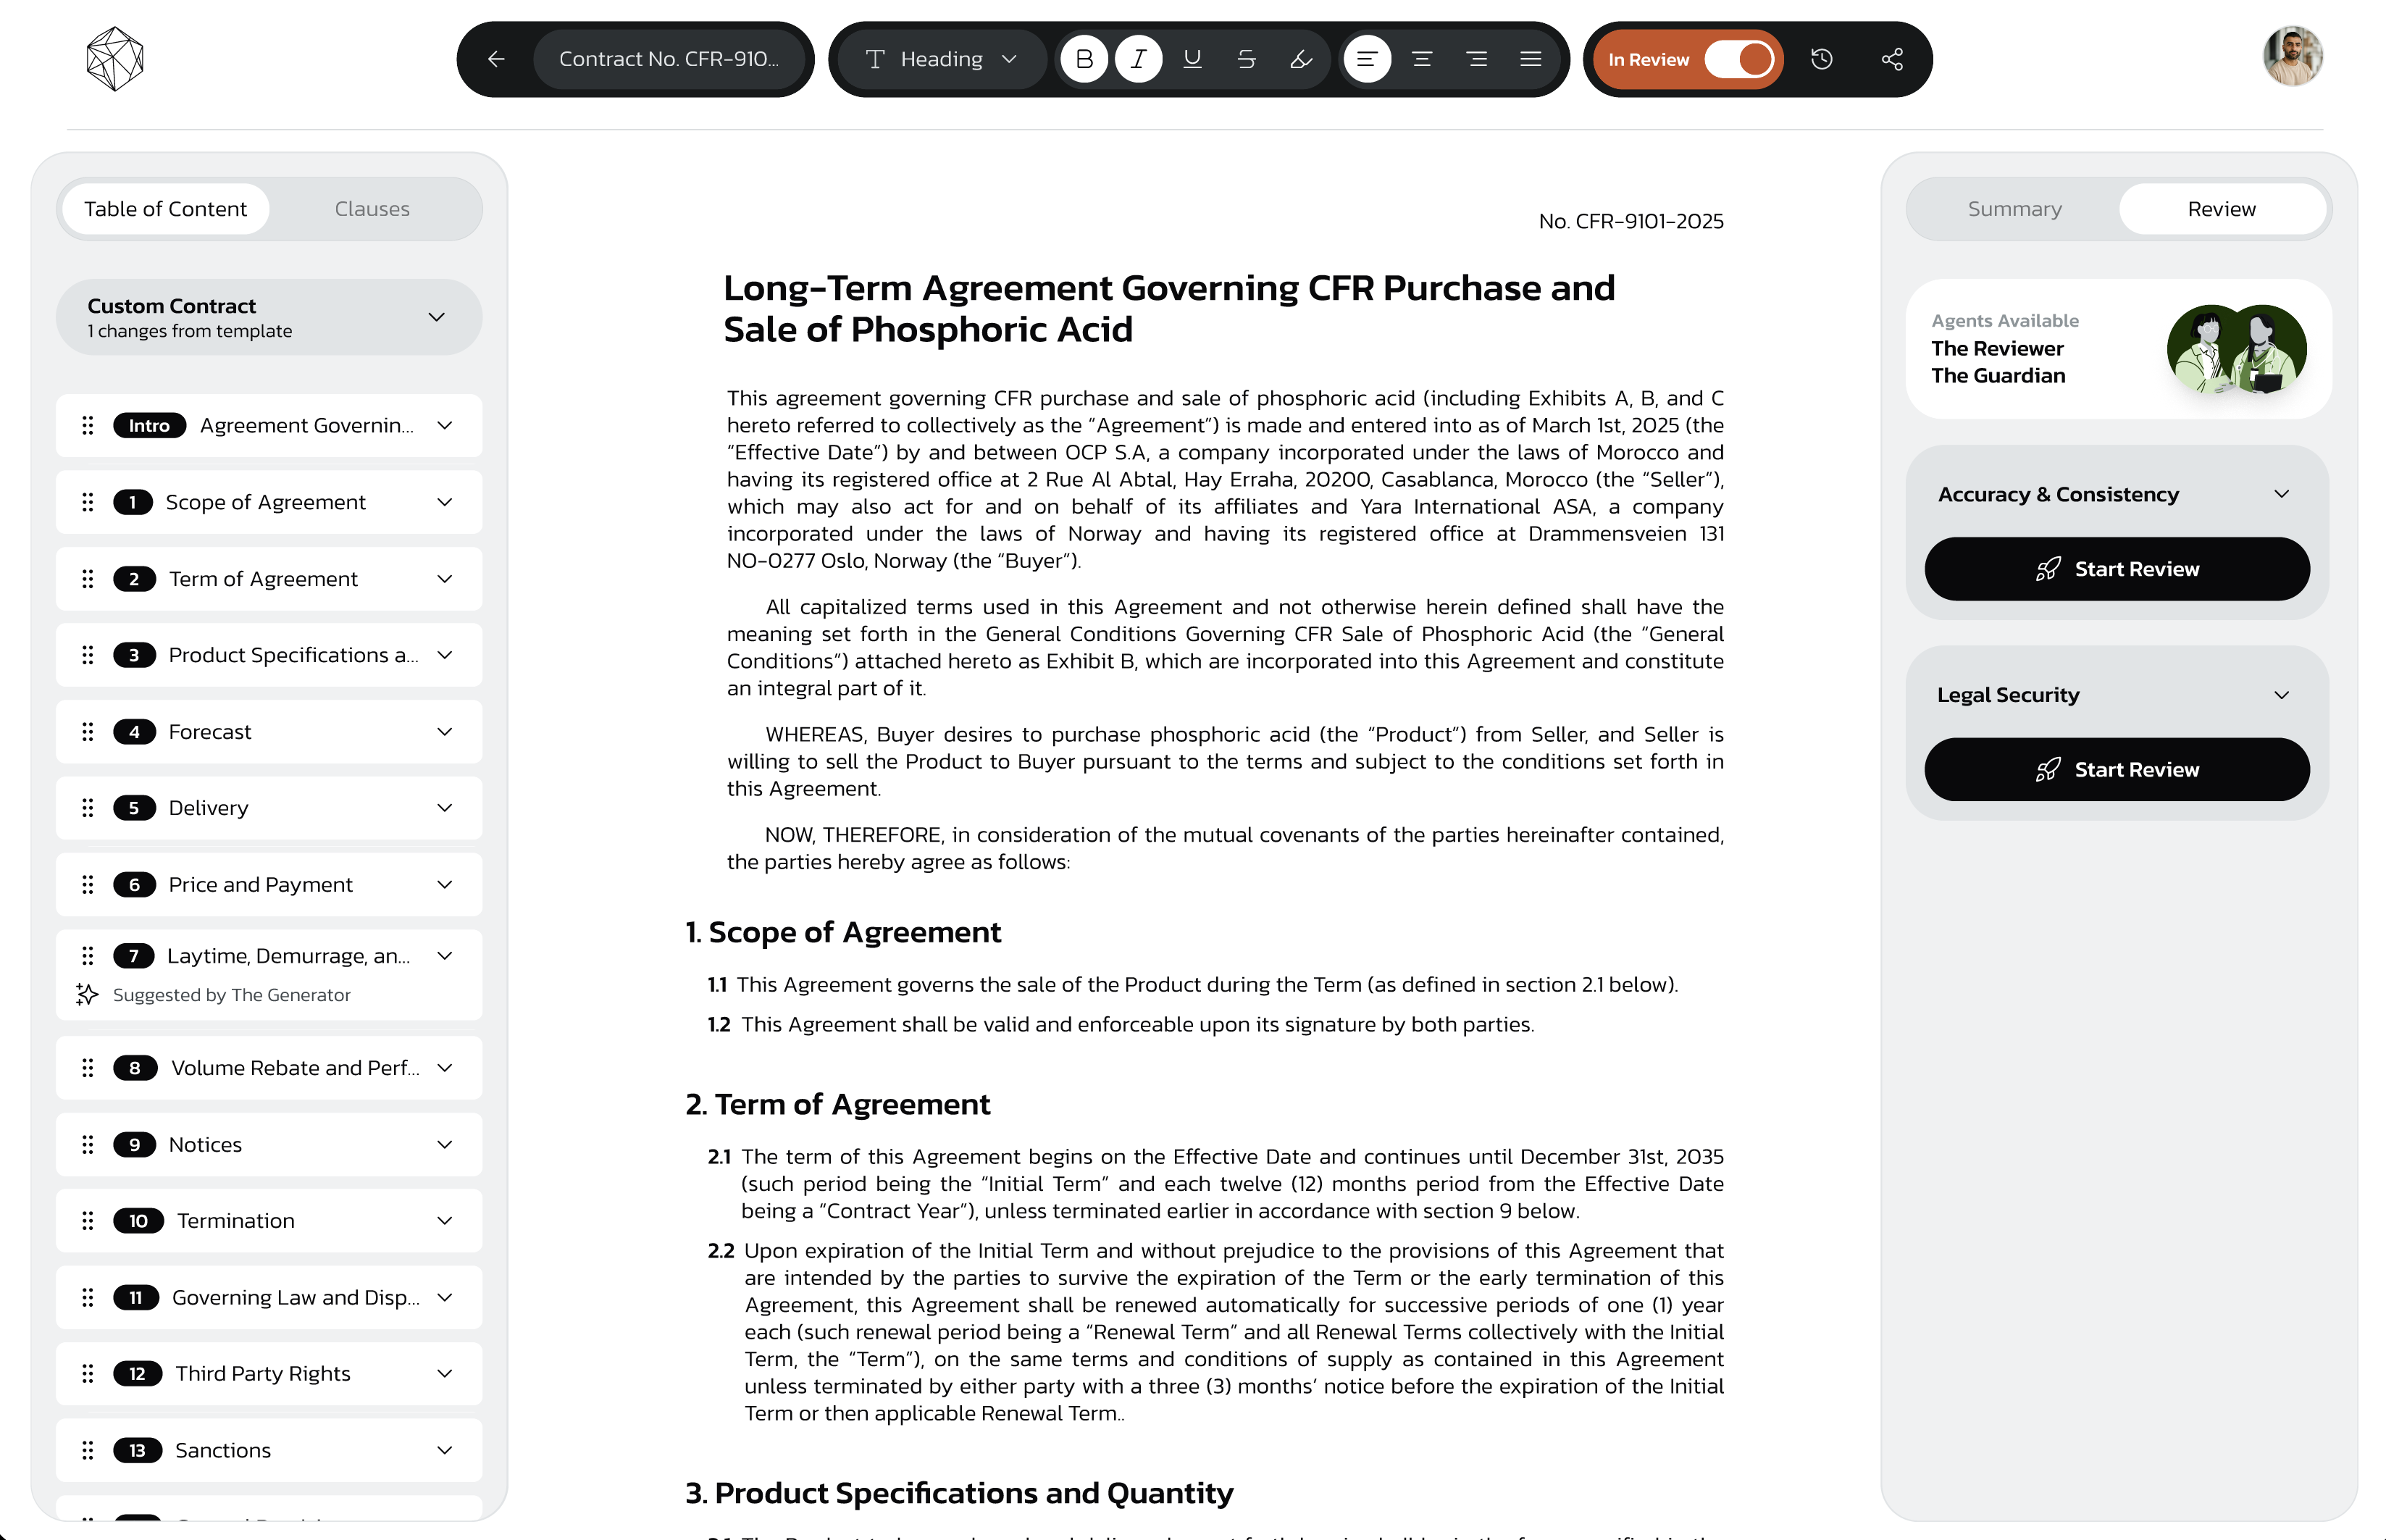
\includegraphics[width=1\textwidth]{Images/Reviewer Agent View.png}
    \captionof{figure}{Contract Review Panel}
    \label{fig:reviewer_agent_view}
\end{center}

\begin{center}
    \centering
    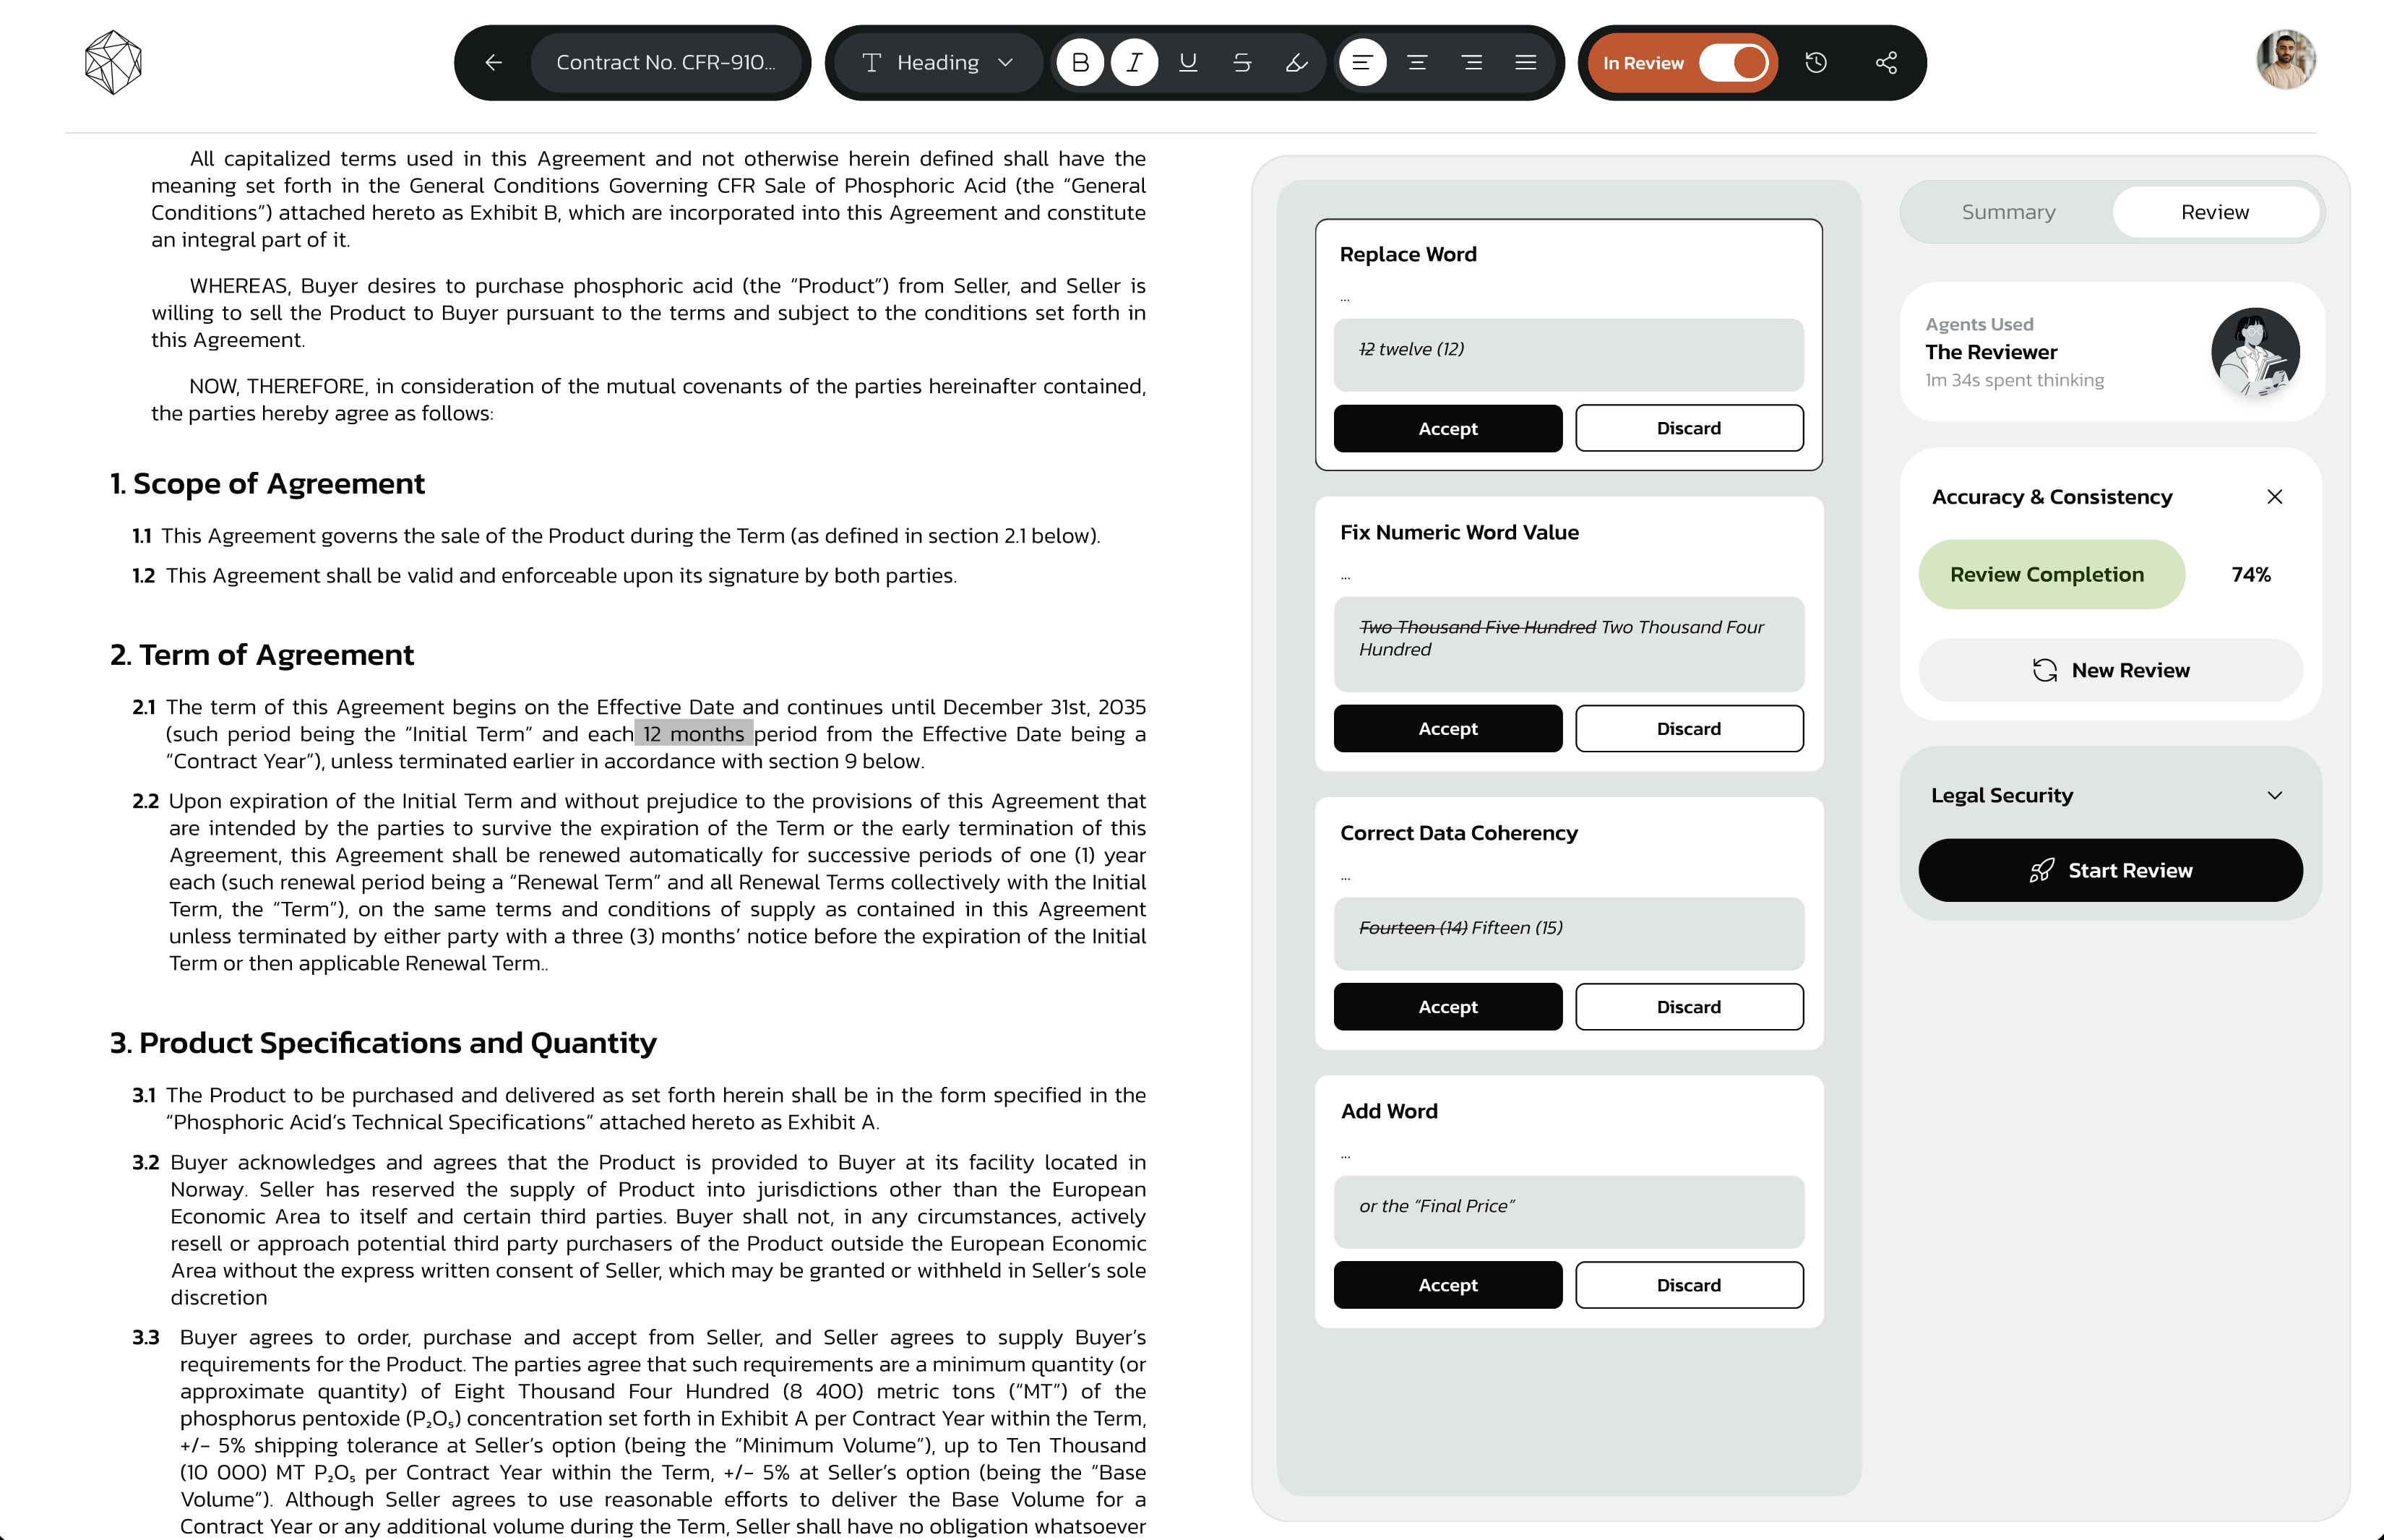
\includegraphics[width=1\textwidth]{Images/Reviewer Agent Result.png}
    \captionof{figure}{Contract Review Results}
    \label{fig:reviewer_agent_result}
\end{center}

% Contract History
\subsection{Contract History}
Users access the contract's History mode via the history button on the navigation bar. This mode automatically tracks each contract modification—triggered by status changes, downloads, or manual saves—while also allowing manual creation of specific versions. Each version is listed chronologically in the right panel, facilitating easy navigation and management.

From this interface, users can perform several key actions:

\begin{itemize}
    \item \textbf{Restore Version:} Reverts the entire contract to a previously saved version.
    \item \textbf{Rename Version:} Allows clear labeling and identification of historical contract states.
    \item \textbf{Paragraph-Level Management:} Enables users to individually restore or copy previous paragraphs into the current document. Restoration replaces current content, while copying appends historical content alongside existing text.
\end{itemize}

The integrated TipTap editor automatically synchronizes all changes, ensuring consistency across all user views.

\begin{center}
    \centering
    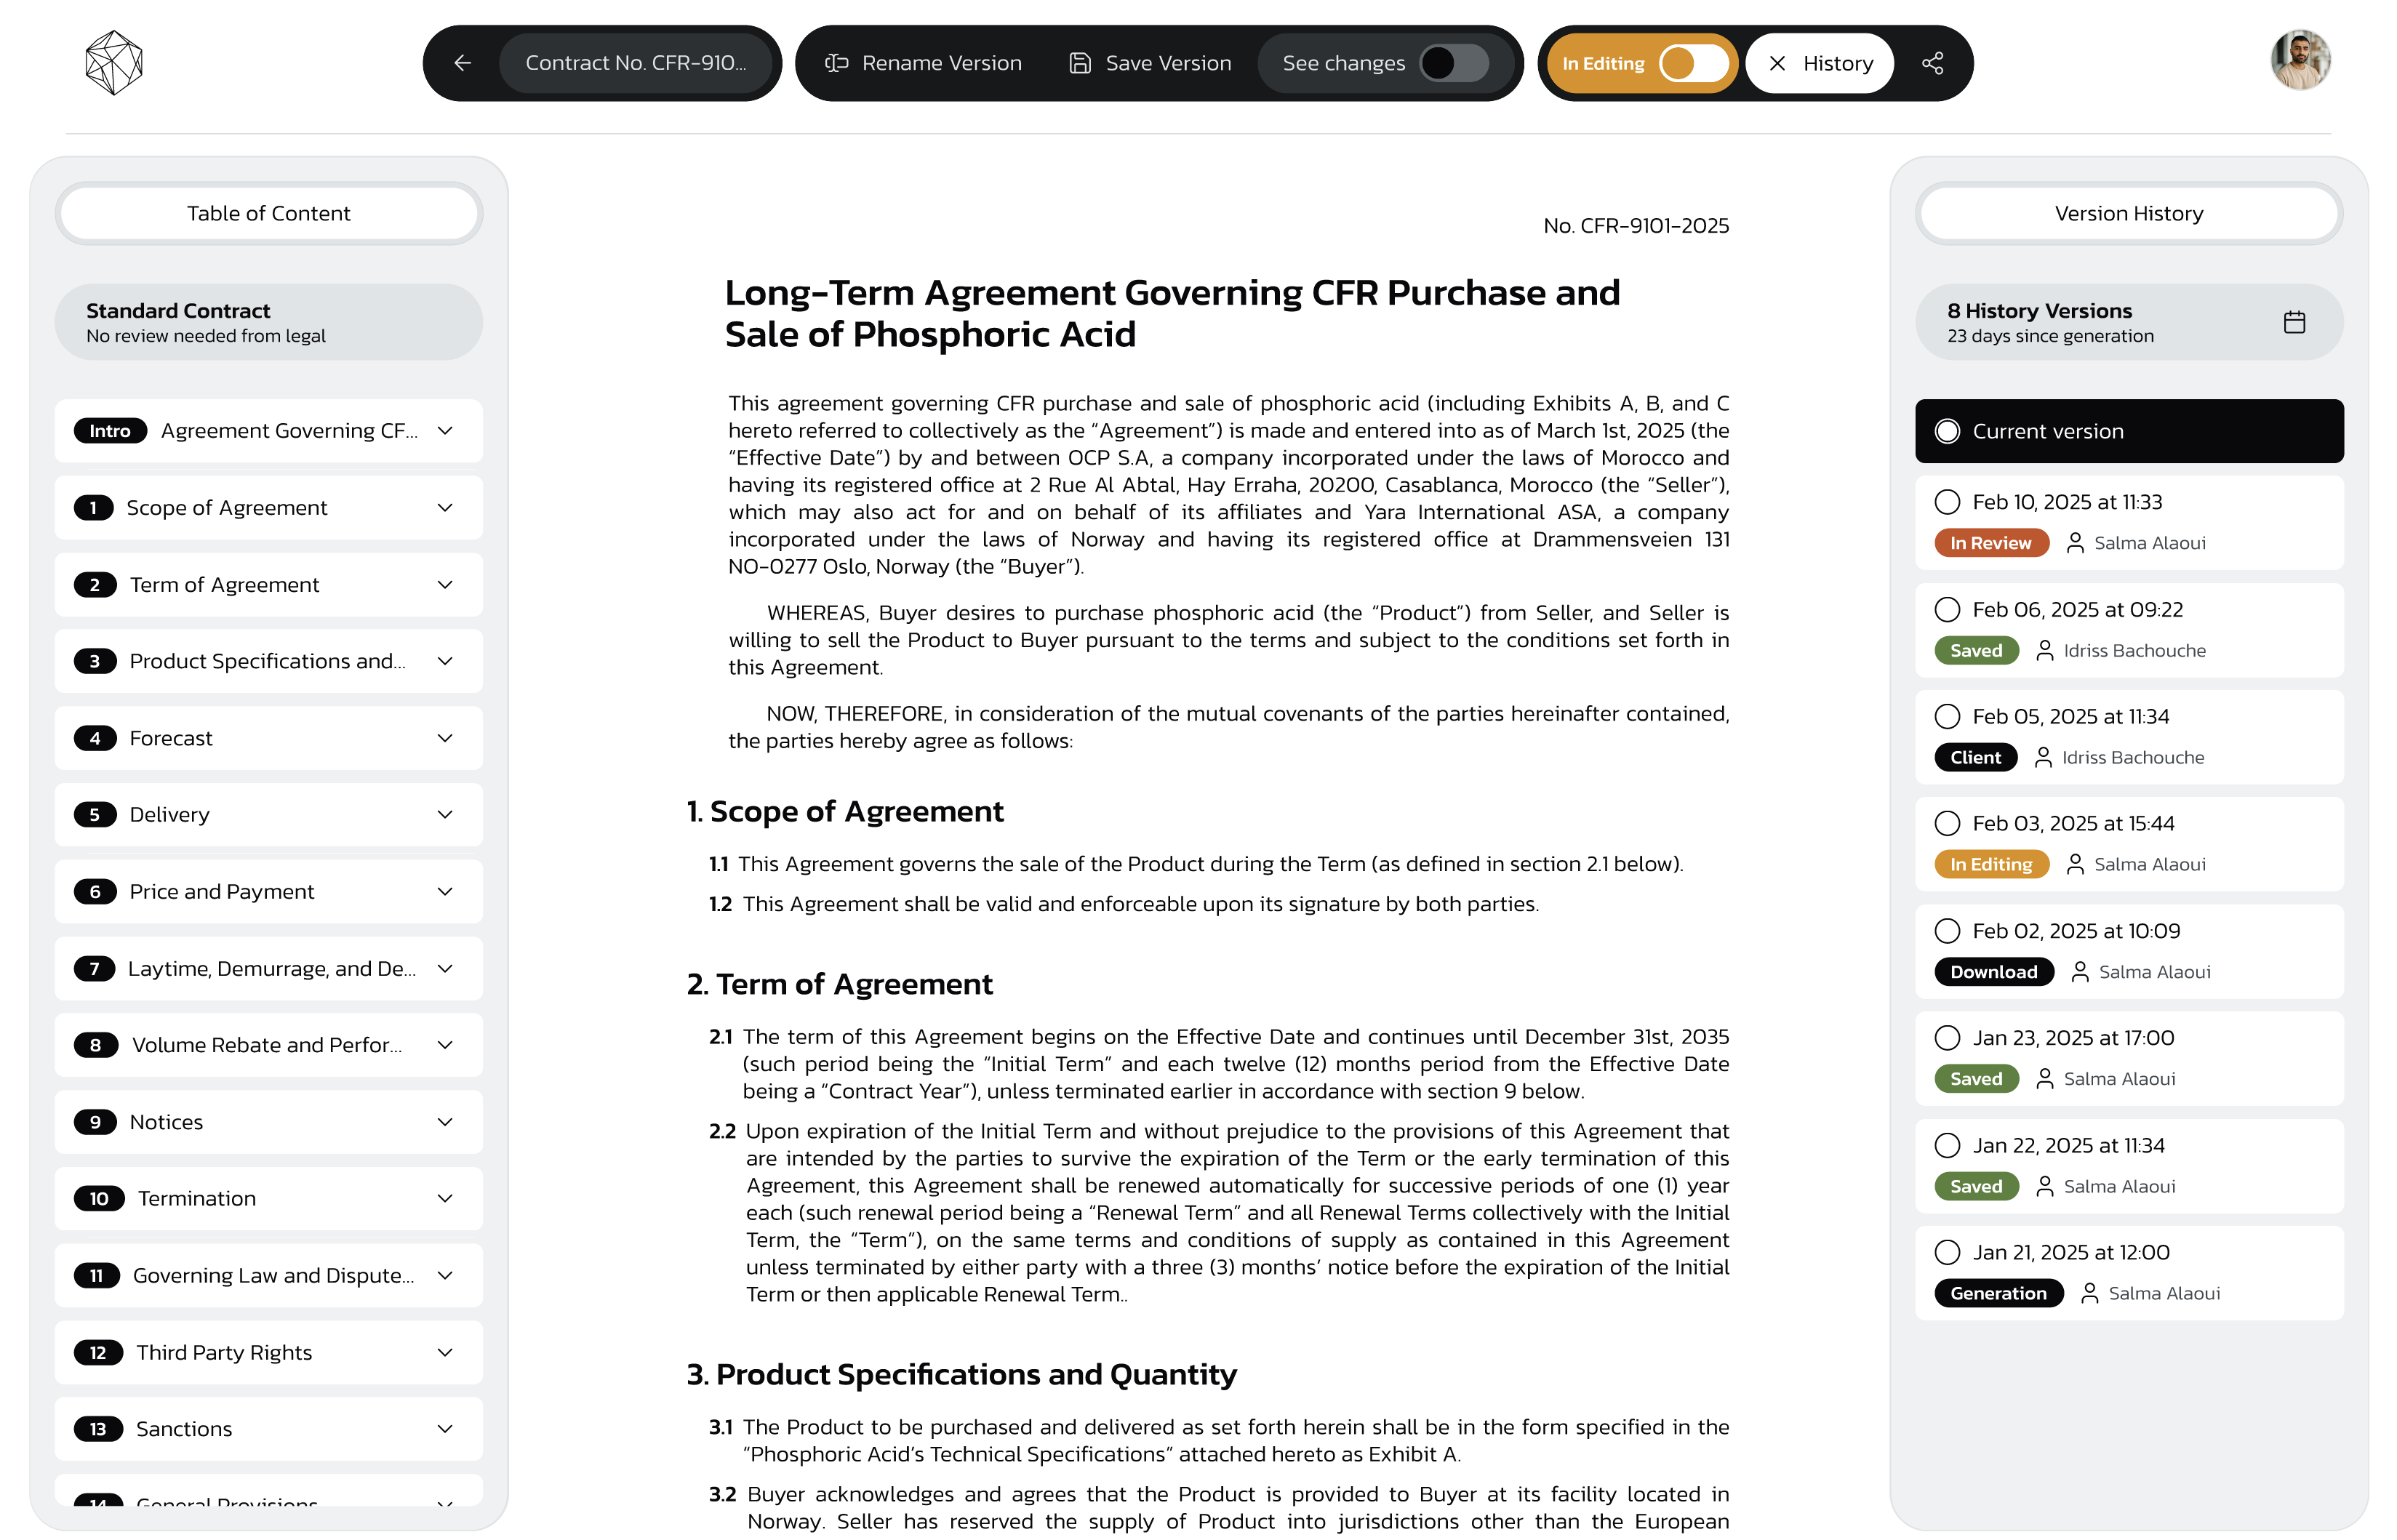
\includegraphics[width=1\textwidth]{Images/Contract History - Contract Versions.png}
    \captionof{figure}{Contract History Interface}
    \label{fig:contract_history_interface}
\end{center}

\begin{center}
    \centering
    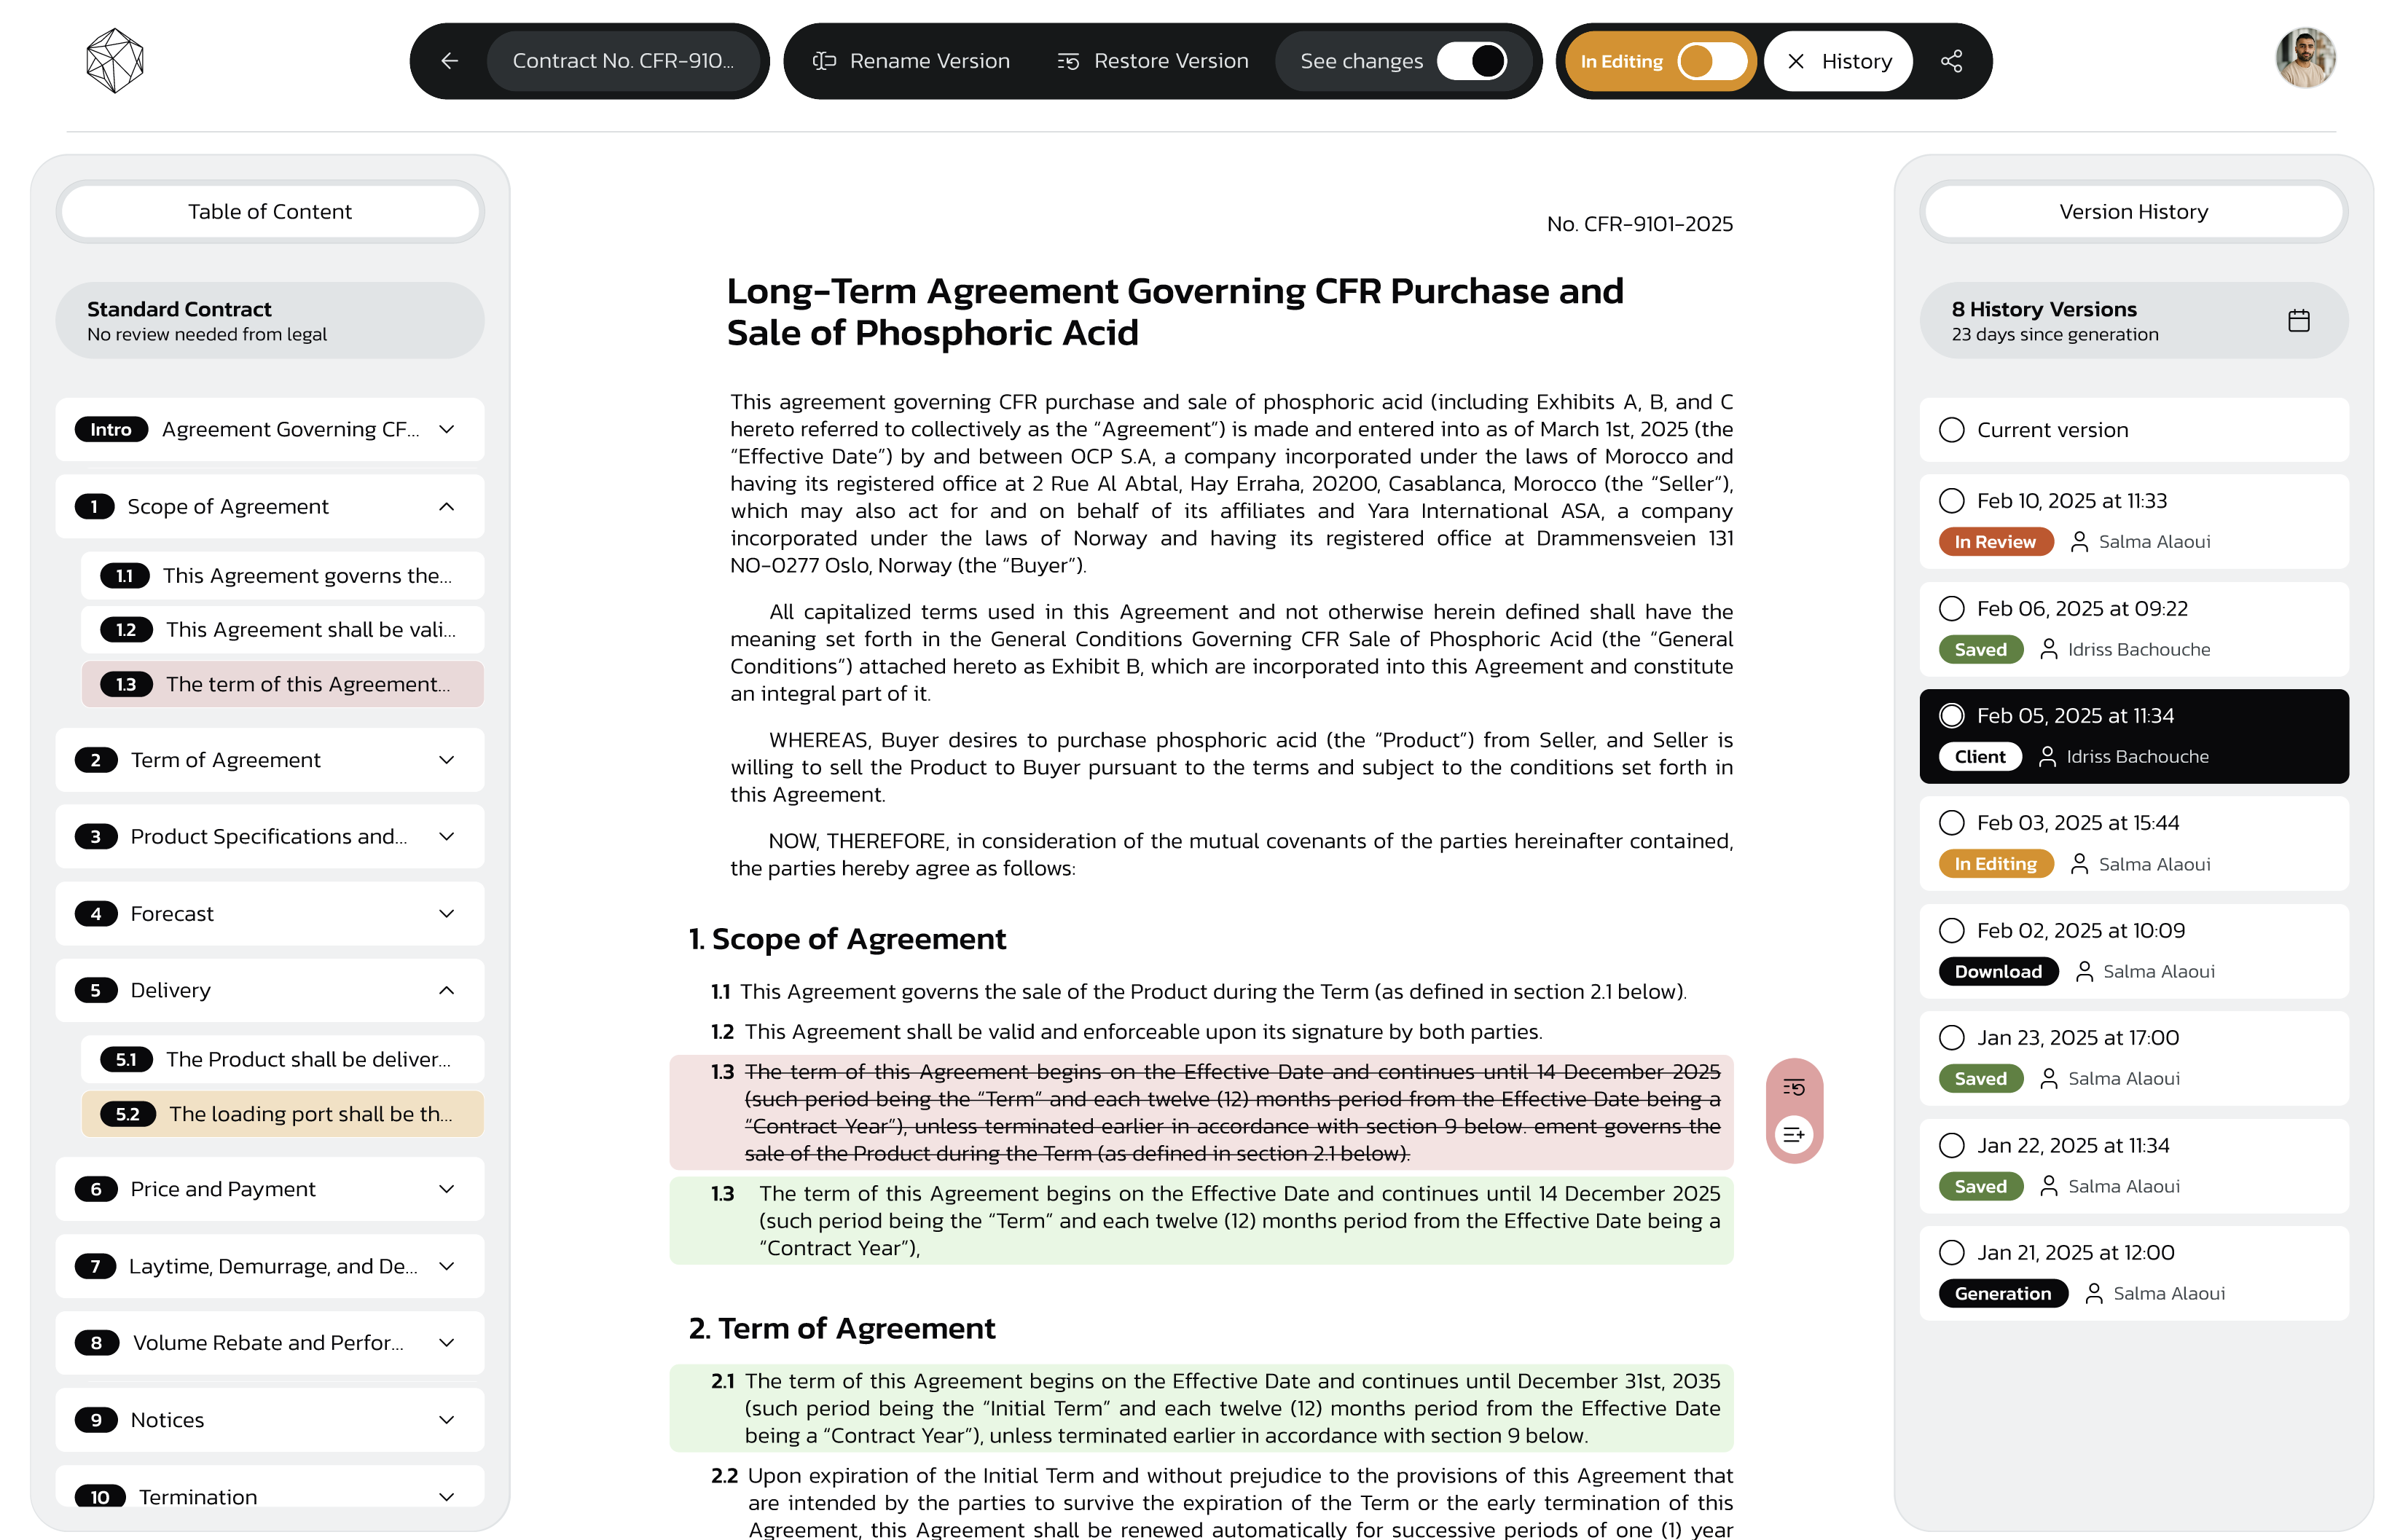
\includegraphics[width=1\textwidth]{Images/Contract History - Paragraph Versions.png}
    \captionof{figure}{Paragraph Version Tracking and Restoration}
    \label{fig:track_changes_across_versions}
\end{center}

% Finalized Contract
\subsection{Finalized Contract}
Upon successful reviews and edits, contracts are finalized, transitioning into the finalized status. Finalized contracts are exportable as PDF/Word documents, shareable via secure links or email attachments, enabling seamless client communications.

\begin{center}
    \centering
    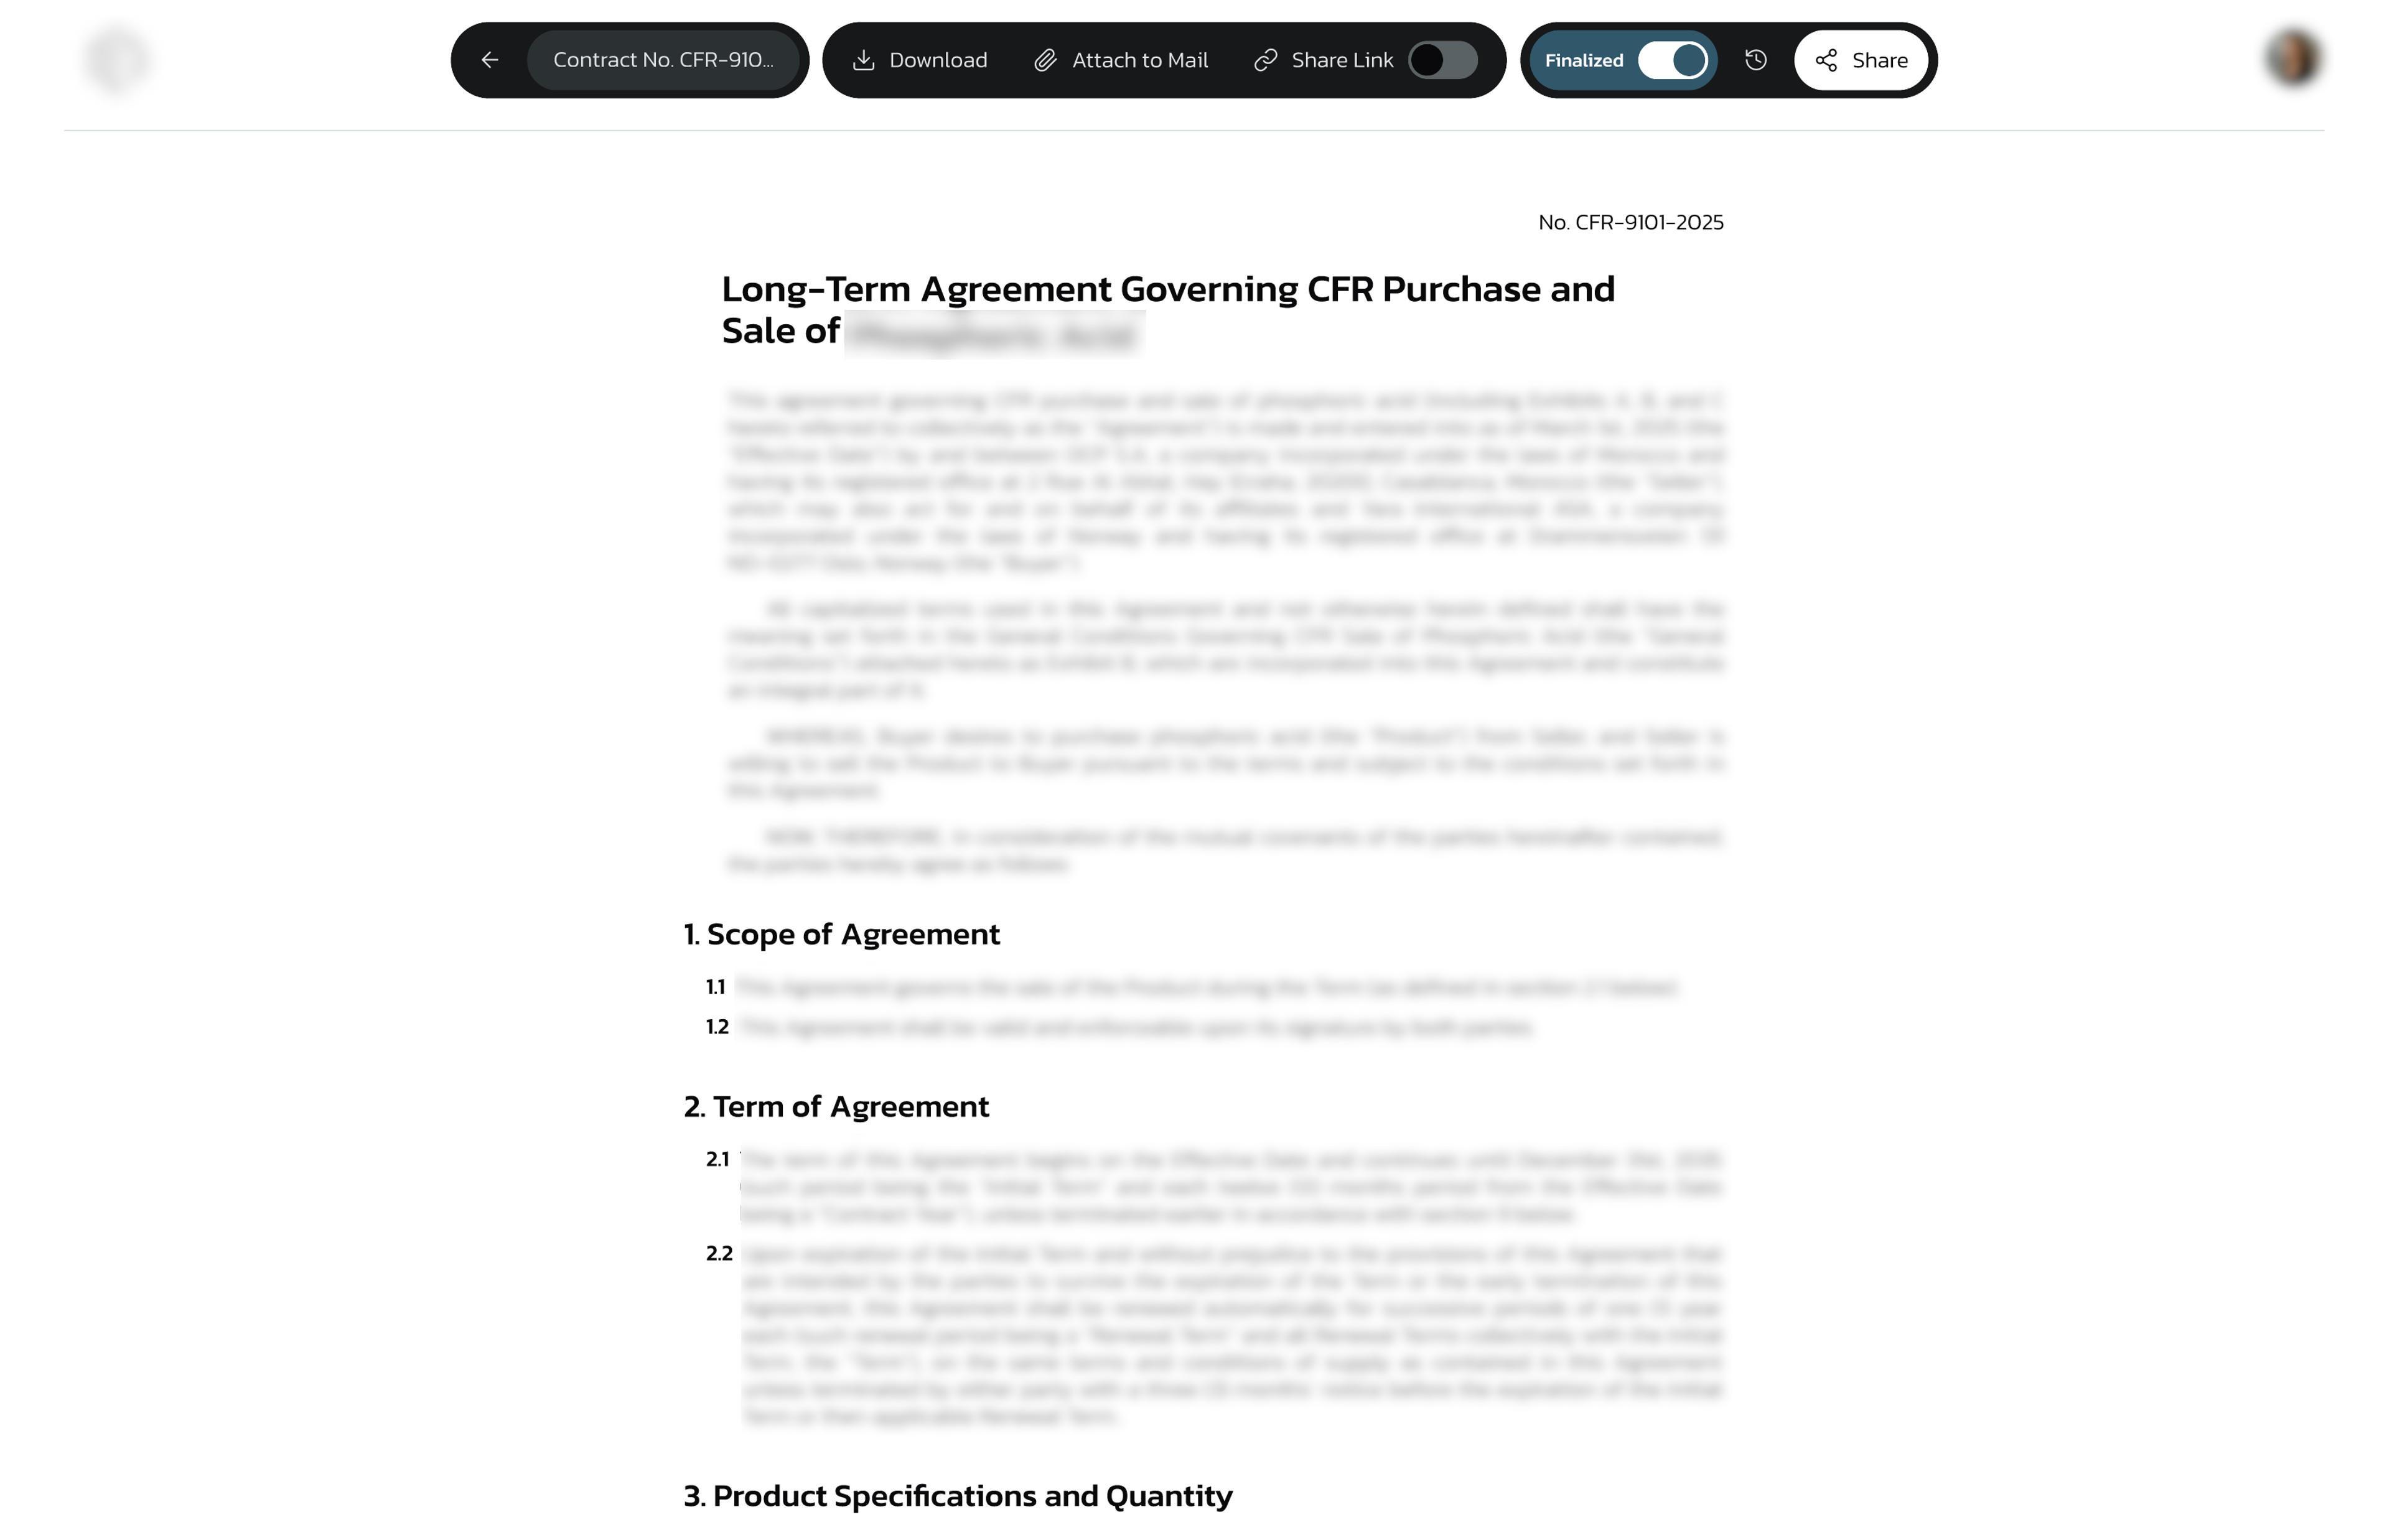
\includegraphics[width=1\textwidth]{Images/Contract Status - Finalized.png}
    \captionof{figure}{Finalized Contract Interface}
    \label{fig:contract_status_finalized}
\end{center}

% Verification of Requirements
\section{Verification of Requirements}
The verification of functional and non-functional requirements is an essential phase in ensuring the developed solution aligns with the initial specifications identified during the analysis phase. This section outlines how the implemented solution satisfies the requirements detailed in Chapter 2.

\subsection{Verification of Functional Requirements}
The intelligent contract management solution underwent systematic verification of its functional capabilities. Initial verification was conducted through iterative demonstrations and regular review meetings with the project stakeholders. These sessions validated critical functionalities including contract generation, clause management, editing capabilities, and AI-assisted contract reviews. Specifically, the Sales and Legal user functionalities were thoroughly tested to ensure seamless user interaction and accurate functional behavior. Remaining functionalities, such as extensive integration testing and further refinement of clause management features, are scheduled for completion within the remaining internship period. While automated unit and integration tests using the designated libraries (Jest and Pytest) are planned, their execution and reporting are scheduled for the final phase of the internship.

\subsection{Verification of Non-Functional Requirements}
The non-functional aspects, crucial for user satisfaction and system reliability, were verified through targeted approaches as follows:

\begin{itemize}
    \item \textbf{Usability:} The platform was designed with an intuitive and familiar interface, inspired by widely used enterprise applications. Initial user feedback, collected from a select group of Sales and Legal users, confirmed that the interface met the usability standards, ensuring a comfortable and efficient user experience.
    \item \textbf{Maintainability:} Regular code reviews and adherence to best practices in software architecture were employed to validate maintainability. The adoption of a modular, service-oriented architecture facilitated easier updates and extensions, allowing new functionalities to be integrated efficiently. Future scheduled unit and integration tests will further ensure system stability and maintainability.
    \item \textbf{Security:} Security verification involved the integration and configuration of Azure Entra ID, ensuring robust authentication and role-based access control. Regular security audits and compliance checks were established to detect and rectify vulnerabilities promptly. Further penetration tests and comprehensive security assessments are planned to maintain and enhance the platform's security posture.
\end{itemize}

% Conclusion
\section{Conclusion}
This chapter has provided an extensive account of the implementation and validation processes of the intelligent contract management platform. We detailed and justified the technology choices across frontend, backend, AI integration, databases, and infrastructure components, ensuring optimal performance, maintainability, and scalability. Furthermore, comprehensive descriptions of the core functionalities—including contract generation, editing workflows, clause management, systematic review processes, and historical tracking—demonstrated alignment with user needs and operational requirements. Finally, the validation processes systematically verified that the platform met all specified functional and non-functional criteria, confirming its robustness, security, usability, and readiness for deployment in real-world scenarios.
